% ============================================================
%  Sections: General · Visual Design · Spatial Design
% ============================================================
\label{chap:design}
This chapter designs the tool from the specification of Chapter~\ref{chap:from-themes-to-requirements}. It moves from \emph{what} students need to \emph{how} the interface answers that need: each section states a decision, the requirement or evidence it answers, and the alternatives it was weighed against. It operates at level~3 of Munzner's nested model, visual encoding and interaction design~\cite{munzner2009}.

Together with Chapter~\ref{chap:implementation}, this chapter answers the second research question:

\begin{quote}
\textit{How can we design and implement a hybrid interface that combines graph-based visualisation with table-based planning to help students plan their studies and understand curriculum structure and course dependencies, based on those requirements?}
\end{quote}

The chapter is therefore organised by design dimension rather than by region of the screen: first the general architecture and the data model it rests on, then the visual encoding of curriculum elements, then interaction, and only then the individual views and features. This follows from the level Munzner's model places the chapter at, whose unit of design is the encoding or interaction technique, and which treats visual encoding and interaction as one level because the two are mutually interdependent~\cite[p.~922]{munzner2009}. An encoding such as the obligation channel, the subject-colour hierarchy or the course lifecycle is a property of the design, not of a panel: the same encoding appears in the Graph View, in the Table View and in the catalogue, and it has to be derived once from the evidence that motivates it rather than three times from wherever it happens to be visible. Organising by screen region would split each of those decisions across the regions that display it. The view- and feature-specific sections that follow the three dimension sections therefore describe only what is genuinely particular to a view or a feature, and refer back to the encodings rather than restating them.

The design decisions presented below are guided by the nine design principles for a study planning assistant in higher education established by Bartel et al.~\cite{bartel_design_2024}, alongside the direct empirical evidence gathered from the formative interviews.

Several decisions of the design originate directly from the Figma prototype used in the formative interviews (Chapter~\ref{chap:formative-study}). These elements were retained on the basis that six independent participant walkthroughs did not surface any objections to them. While this absence of objection provides indirect evidence that a concept is at least not actively unsuitable, it is acknowledged as weaker support than an explicit user requirement grounded in a stated need. Each assumption is discussed exactly where it applies in this chapter, clearly distinguishing between what was carried forward unchallenged and what was actively changed in response to feedback.

The tool's scope follows directly from Chapter~\ref{chap:methodology} and~\ref{chap:from-themes-to-requirements}, so all five OOS boundaries (Section~\ref{sec:overall-scope}) are already-settled inputs to design, not decisions this chapter makes or reconsiders. For each decision below, the rationale is stated explicitly exactly where the interface decision is discussed. These rationales are grounded in a feature or requirement, a prototype assumption not criticised during the formative interviews, common design knowledge, or specific published literature (such as Bartel et al.~\cite{bartel_design_2024} principles or Nielsen's usability heuristics~\cite{nielsen1994}). Where a genuine alternative was weighed during design, it is recorded alongside its rejection reason; not every decision below had a live alternative worth naming, so this is not claimed uniformly.

% ============================================================

\section{General Architecture and Data Model}
\label{sec:general}
This section establishes the frame every later section builds on, and moves from the outside inwards. It first divides the screen into panels, then settles what occupies the centre panel and why only one view may occupy it at a time. Its last two subsections leave the screen and describe the data model instead: the curriculum structure and the course obligation categories the interface is given to display. They are placed here because they are inputs to every visual encoding and every compliance rule in the later sections, which name their categories and cannot be derived without them.

% ------------------------------------------------------------
\subsection{Three-Panel Shell}
\label{sec:three-panels}
The outermost design decision is how the screen is divided, because that division fixes where every component described later in this chapter lives. Participants described planning as analogous to working at a physical desk (\enquote{like a desk… you just push things around} (T21)), which presupposes simultaneous access to multiple activities rather than sequential navigation between them. Feature~\ref{feat:004}, Req.~1 requires that the catalogue and the planning canvas be simultaneously visible, so a course can be added while observing the canvas update. Feature~\ref{feat:003}, Req.~1 requires compliance feedback to update in real time, ruling out placing it behind a tab where it would stop being ambient. Nielsen's recognition-rather-than-recall heuristic~\cite{nielsen1994} calls for minimising the user's memory load. A fixed region per function satisfies this directly: its position is stable, so a student recognises where a function lives instead of having to recall which mode a shared region currently holds.

Based on this evidence, the interface is divided into three spatially fixed, simultaneously visible panels (Figure~\ref{fig:three-panels}): a left panel offering three context-sensitive modes (Course Catalogue in Table View, filter controls in Graph View, and the independently-toggleable \gterm{recommendation-panel}{Recommendation Panel}), a centre panel hosting the active canvas (Table or Graph View), and a right panel hosting the Dashboard, which reports compliance and progress regardless of the active view. The sidebar-plus-canvas half of this structure is carried forward from the prototype unchanged; the two genuine additions are the right-panel Dashboard, which did not exist in the prototype (obligation was shown only as inline node indicators there) and was added in direct response to Feature~\ref{feat:003}, Req.~1, and the independent Recommendation Panel, in response to Feature~\ref{feat:012}, Req.~2.

A \emph{tab-based layout} was rejected because it makes the catalogue and the canvas mutually exclusive, which Feature~\ref{feat:004}, Req.~1 forbids, and a \emph{modal Dashboard} because compliance feedback surfaced only on request would let violations accumulate silently. The Recommendation Panel's placement is discussed in Section~\ref{sec:rec-panel}.

\begin{figure}[htbp]
\centering
\begin{tikzpicture}[font=\small, scale=0.88, transform shape]
  % Left panel (Widened to 2.8 to prevent text cutoff)
  \fill[panelgray, rounded corners=4pt] (0,0) rectangle (2.8,5.5);
  \draw[gray!50, rounded corners=4pt, line width=0.7pt] (0,0) rectangle (2.8,5.5);
  \node[font=\footnotesize\bfseries] at (1.4,5.15) {Left Panel};
  
  % Adjusted Y-coordinates down to prevent overlap with the heading
  \node[text width=2.6cm, align=center, font=\scriptsize] at (1.4,4.2)
    {Course Catalogue\\\textit{(Table View)}};
  \draw[gray!30, dashed, line width=0.5pt] (0.2,3.5) -- (2.6,3.5);
  
  \node[text width=2.6cm, align=center, font=\scriptsize] at (1.4,2.8)
    {Filter Controls\\\textit{(Graph View)}};
  \draw[gray!30, dashed, line width=0.5pt] (0.2,2.1) -- (2.6,2.1);
  
  % Forced line breaks to ensure 'Recommendation' fits nicely
  \node[text width=2.6cm, align=center, font=\scriptsize] at (1.4,1.3)
    {Recommendation\\Panel\\\textit{(independent toggle)}};

  % Centre panel (Adjusted start/end to accommodate wider side panels)
  \fill[white, rounded corners=4pt] (2.95,0) rectangle (8.05,5.5);
  \draw[gray!50, rounded corners=4pt, line width=0.7pt] (2.95,0) rectangle (8.05,5.5);
  \node[font=\footnotesize\bfseries] at (5.5,5.15) {Centre Panel};
  \node[text width=4.8cm, align=center, font=\scriptsize] at (5.5,4.3)
    {Table View \textit{or} Graph View\\(active canvas)};
  \fill[gray!15, rounded corners=3pt] (3.8,0.25) rectangle (7.2,0.75);
  \draw[gray!40, rounded corners=3pt, line width=0.5pt] (3.8,0.25) rectangle (7.2,0.75);
  \node[font=\scriptsize] at (5.5,0.5) {Table \quad $|$ \quad Graph};

  % Right panel (Shifted right to accommodate wider left panel)
  \fill[panelgray, rounded corners=4pt] (8.2,0) rectangle (11.0,5.5);
  \draw[gray!50, rounded corners=4pt, line width=0.7pt] (8.2,0) rectangle (11.0,5.5);
  \node[font=\footnotesize\bfseries] at (9.6,5.15) {Right Panel};
  \node[text width=2.6cm, align=center, font=\scriptsize] at (9.6,4.3)
    {Dashboard\\\textit{(compliance and progress)}};
\end{tikzpicture}
\caption{Three-panel shell. The left panel's catalogue and filter controls follow the active view, while the Recommendation Panel toggles independently. Centre: the active canvas. Right: the Dashboard.}
\label{fig:three-panels}
\end{figure}

\subsection{Graph and Table View: Mutually Exclusive Centre Panel}
\label{sec:mutual-exclusion}
Within that shell, the centre panel is where planning happens, and the next two subsections settle which view occupies it and what both are drawn on. Both views compete for the same resource, horizontal space, and for different reasons: the Graph View needs width to show the curriculum tree at legible node sizes, the Table View to give every semester a column wide enough for its course cards. At standard screen widths there is not enough of it for both at a usable scale. Participants themselves differentiated the two views by purpose: \enquote{graph used for exploration, not planning} (T20), which supports mutual exclusivity rather than permanent co-display.

Based on this, only one, Table View or Graph View, occupies the centre panel at any time. This division of labour, Graph View for exploration, Table View for commitment, was already present in the prototype (Chapter~\ref{chap:formative-study}) and was not questioned by any formative-study participant. The active view is toggled by a control in the toolbar.

A \emph{split-screen layout}, with the two views side by side, was rejected for the reason just given: neither retains usable width. A second alternative was a \emph{minimap or preview} of the inactive view. This was also rejected: a preview detailed enough to be informative would have required rendering a substantial second view, effectively reintroducing the space constraints of a split-screen layout. Conversely, a reduced preview that avoided these constraints provided too little information to justify its presence.

% ------------------------------------------------------------
\subsection{Unified Interactive Canvas for Both Views}
\label{sec:canvas}
Whichever of the two is active, it is drawn on the same surface. Spatial metaphors recurred when participants described planning: \enquote{like a desk… you just push things around} (T21), \enquote{I'd rather place them how I want} (T28). A static, column-sorted table cannot express spatial priority, distance-based de-emphasis, or personal groupings that participants explicitly requested (T28, T29). Feature~\ref{feat:013}, Req.~1 (free grouping) and Feature~\ref{feat:013}, Req.~2 (positions persist) require the canvas to hold arbitrary item positions. Direct manipulation replaces command syntax with action on the objects of interest themselves, kept visible and reversible~\cite{shneiderman1983}; dragging a course card into a semester is that action, where a form would be the syntax.

Based on this, both the Table View and the Graph View are rendered on an \emph{interactive, pannable, zoomable canvas}. Items (course, modules, table, graph structure) are positioned as absolute objects on the canvas. Users navigate by panning (scrolling the canvas in any direction) and zooming. Dragging items updates their position in real time. A configurable snap grid enforces positional alignment after a drag gesture for the Table View, producing ordered layouts without demanding fine motor precision. The visual representation of any item is identical in both views; sharing the same canvas model for both means the item definition is authored once (Feature~\ref{feat:004}, Req.~4: two-way synchronisation), eliminating the risk of visual inconsistency between views.

% ------------------------------------------------------------
\subsection{Curriculum Abstraction}
\label{sec:curriculum-abstraction}

Participants in the formative interviews described manual curriculum extraction from TISS, TU Wien's course and curriculum information system, as burdensome and error-prone: \enquote{clicking through TISS… pulling it out manually} (T37), \enquote{very error-prone… you might slip in the row} (T62). Relying on students to manually input and structure their own data violates Bartel et al.~\cite{bartel_design_2024} principle of \emph{centralisation of systems and information}, which argues against forcing students to cross-reference multiple decentralised sources like official PDFs. Furthermore, Feature~\ref{feat:003} requires curriculum compliance rules to operate on named, semantically meaningful categories (modules, exam subjects). Guided additionally by Bartel et al. principles of \emph{study-programme-specific personalisation} and the \emph{use of university identifiers}, the tool's data architecture ensures these categories are not generic; they must match the exact structural hierarchy of the specific study programme and utilise official university terminology.

Consequently, all curriculum data (programme structure, module composition, course list, ECTS values, obligation types, estimated weekly hours) is provided directly to the system. This imported data explicitly includes the official university abbreviations and course numbers, which are widespread among students and essential for fast, familiar information retrieval. 

To achieve this programme-specific tailoring without requiring manual setup, the imported curriculum is abstracted as a strict four-level hierarchy: 

Programme $\to$ Exam Subject $\to$ Module $\to$ \gterm{course}{Course Item}. 

This hierarchy is encoded as a fixed design constraint to perfectly match the institutional structure of the TU Wien programmes covered (Section~\ref{sec:overall-scope}; Figure~\ref{fig:curriculum-hierarchy}). A module containing exactly one Course Item is collapsed to that Course Item in the interface; an intermediate layer containing nothing but itself would add a hierarchy step without conveying information. OOS2 (Chapter~\ref{chap:methodology}) fixes the planning granularity at course-within-semester, which makes the Course Item the foundational level of this hierarchy.

Underpinning this user-facing data, every element of the hierarchy also carries a stable internal identifier that persists across data refreshes and across both views, ensuring that user selections remain stable (Feature~\ref{feat:001}, Req.~2). While the structural hierarchy and core curriculum data are strictly fixed, the system provides one minor exception: it allows students to manually override a course's term availability in their personal plan. This localised flexibility is necessary because actual course offerings change from year to year faster than a periodically-refreshed dataset can reliably track. 

Alternative data models were considered but rejected due to their inability to support automated compliance tracking. A \emph{flat course list} (with no structural hierarchy) was rejected because compliance rules explicitly reference modules and exam subjects as named, verifiable categories; a flat list fundamentally cannot represent these groupings. Similarly, a \emph{three-level hierarchy} (omitting the Exam Subject level) was rejected because the Compliance Engine must evaluate ECTS quotas at the exam-subject level, which represents a critical institutional constraint.


\subsection{Course Obligation Abstraction}
\label{sec:course-obligation-abstraction}

Driven by the same need for \emph{study-programme-specific personalisation}~\cite{bartel_design_2024} that motivated the structural hierarchy, the system must also accurately encode the rules governing which courses are required versus optional. To achieve this, the underlying abstraction was designed to accommodate the unique rules of both degree programmes defined in the tool's scope (Section~\ref{sec:overall-scope}) simultaneously, rather than being extracted from one programme and merely applied to the other. 

This unified approach is necessary because the two covered programmes define their obligation taxonomies differently. In the Bachelor programme, unmarked modules are \emph{Pflichtmodule} (mandatory); modules marked~(+) are \emph{Wahlmodule der engen Wahl} (quota-based narrow-choice electives); and modules marked~(*) are \emph{Wahlmodule der breiten Wahl} (broad-choice electives). In the Master programme, unmarked modules are likewise \emph{Pflichtmodule}, but modules marked~(+) are \emph{Core-Module}, acting as a gating condition rather than a separately countable requirement; modules marked~(*) are \emph{Wahlmodule}, selectable only once that core gate is satisfied. 

Because obligation types cannot be reduced to a single flat enumeration shared across both programmes, the underlying data model encodes these programme-specific semantics separately. However, to maintain a unified user experience, it exposes them uniformly at the interface level as a single three-tier encoding: \emph{mandatory / constrained elective / fully elective} (introduced in Section~\ref{sec:obligation}). For example, the Bachelor's quota-gated \emph{enge Wahl} and the Master's completion-gated \emph{Core} both surface as \emph{constrained electives}, since both impose a structural precondition beyond free choice. The abstraction was built to carry both programmes at once, and it does; how far it would carry beyond the two is untested here and is taken up in the Discussion (Chapter~\ref{chap:discussion}).

Furthermore, the system must handle alternative course formats without breaking these compliance and obligation rules. A small number of modules are officially offered in two structural formats: an integrated lecture-exercise course (VU) or a split lecture-plus-exercise pair (VO~+~UE). Both variants inherit the parent module's single obligation category. When a student selects one variant, the system automatically treats the alternative as satisfied, ensuring the module cannot be double-counted under two different course codes. The recommendation engine (Section~\ref{sec:rec-types-evidence}) is similarly designed to recognise these variant pairs, ensuring that a course already covered by an added variant is never redundantly recommended.

\begin{figure}[htbp]
\centering
\begin{tikzpicture}[
  box/.style={draw=gray!50, fill=gray!15, rounded corners=3pt, minimum width=2.0cm,
              minimum height=0.55cm, align=center, font=\scriptsize, inner sep=3pt},
  prog/.style={box},
  subj/.style={box},
  modul/.style={box},
  cours/.style={box},
  eg/.style={-{Stealth[length=4pt]}, gray!60, thin},
  dots/.style={font=\scriptsize, text=black}
]
  % 1st Level
  \node[prog]  (prog) at (0,-0.1)   {Programme};
  
  % 2nd Level
  \node[subj]  (sa)   at (3.5, 1.2) {Exam Subject A};
  \node[subj]  (sb)   at (3.5,-1.4) {Exam Subject B};
  
  % 3rd Level (Modules OR Collapsed Single Courses)
  \node[modul] (m1)   at (7.0, 2.0) {Module 1};
  \node[modul] (m2)   at (7.0, 0.4) {Module 2};
  
  \node[cours] (c5)   at (10.5,-1.0) {Course};
  \node[cours] (c6)   at (10.5,-1.8) {Course};
  
  % 4th Level (Standard Courses)
  \node[cours] (c1)   at (10.5, 2.4) {Course};
  \node[cours] (c2)   at (10.5, 1.6) {Course};
  \node[cours] (c3)   at (10.5, 0.8) {Course};
  \node[cours] (c4)   at (10.5, 0.0) {Course};
  
  % Edges from Programme
  \draw[eg] (prog.east) -- (sa.west);
  \draw[eg] (prog.east) -- (sb.west);
  
  % Edges from Exam Subjects
  \draw[eg] (sa.east)   -- (m1.west);
  \draw[eg] (sa.east)   -- (m2.west);
  \draw[eg] (sb.east)   -- (c5.west);
  \draw[eg] (sb.east)   -- (c6.west);
  
  % Edges from Modules to Courses
  \draw[eg] (m1.east)   -- (c1.west);
  \draw[eg] (m1.east)   -- (c2.west);
  \draw[eg] (m2.east)   -- (c3.west);
  \draw[eg] (m2.east)   -- (c4.west);
  
  % Column Labels
  \node[font=\tiny] at (0,-2.95)    {Programme};
  \node[font=\tiny] at (3.5,-2.95)  {Exam Subject};
  \node[font=\tiny] at (7.0,-2.95)  {Module};
  \node[font=\tiny] at (10.5,-2.95) {Course};

  % The two single-course modules: the module node is not drawn, so the edge
  % from the exam subject crosses the module column to reach the course.
\end{tikzpicture}
\caption{Four-level curriculum hierarchy. Modules holding several courses keep their intermediate node; a module holding exactly one course is not drawn, and its course attaches directly to the exam subject.}
\label{fig:curriculum-hierarchy}
\end{figure}

\section{Visual Design of Curriculum Elements}
\label{sec:visual}
A recurring theme of the formative interviews was a preference for icon- and colour-based communication over text, T54 reporting that \enquote{too much text is off-putting}. Feature~\ref{feat:011}, Req.~1 records this as the requirement for a \emph{visual-first, low-text} interface, and the encodings below are how the design meets it: each carries on a visual channel what a card would otherwise have to spell out, with text kept as a redundant confirmation.

% ------------------------------------------------------------

\subsection{Course Obligation Encoding}
\label{sec:obligation}

Obligation type was named as a primary filter dimension: \enquote{mandatory… narrow elective… broad elective} (T42). Obligation type must be readable on every card without opening any popover, because it is the most common criterion for deciding whether to explore a course further.

Based on Section~\ref{sec:course-obligation-abstraction}, a course or a module can have three obligation types: mandatory, constrained elective, fully elective (Figure~\ref{fig:obligation-rings}). This is encoded in border weight, an ordered channel of three steps: a thick border denotes mandatory, a medium border constrained elective, and a thin border fully elective. A short text label naming the obligation category is additionally shown in the card footer, again as a secondary, redundant confirmation rather than the primary channel.

Border thickness as the primary channel is also a change from the prototype (Section~\ref{sec:prototype-elicitation}), not a carried-forward assumption: the prototype's obligation indicator was a visible letter badge (M/C/E) directly on each node, with border thickness introduced here instead and a text label introduced as the secondary confirmation just described. This shift is not traceable to a specific interview statement about obligation encoding itself, but it is a direct application of the visual-first, low-text principle (T54, Feature~\ref{feat:011}, Req.~1): a border-weight difference is read pre-attentively, while a letter requires serial reading.

A \emph{multiple concentric border rings} treatment (e.g.\ one ring for elective, two for constrained, three for mandatory, rather than one border of varying thickness) was considered and rejected: adding rings either grows the card outward, which conflicts with the fixed card geometry the snap-grid and table layout depend on, or grows inward at the expense of interior content space, and beyond two rings the count becomes hard to distinguish at a glance at typical card sizes. A single border of varying thickness avoids both problems.
\begin{figure}[htbp]
\centering
\begin{tikzpicture}[font=\scriptsize, scale=0.85, transform shape]
  \def\cw{2.4}\def\ch{2.8}\def\rc{subjectblue}

  % Broad Elective — thin ring
  \fill[white, rounded corners=3pt] (0,0) rectangle (\cw,\ch);
  \draw[\rc, line width=1.0pt, rounded corners=3pt] (0,0) rectangle (\cw,\ch);
  \node[font=\scriptsize\bfseries,text width=2.8cm,align=center] at (1.2,-0.4) {Fully Elective};
  \node[font=\tiny] at (1.2,-0.95) {thin border};

  % Core/Narrow Elective — medium ring
  \def\ox{3.6}
  \fill[white, rounded corners=3pt] (\ox,0) rectangle (\ox+\cw,\ch);
  \draw[\rc, line width=2.0pt, rounded corners=3pt] (\ox,0) rectangle (\ox+\cw,\ch);
  \node[font=\scriptsize\bfseries,text width=2.8cm,align=center] at (\ox+1.2,-0.4) {Constrained Elective};
  \node[font=\tiny] at (\ox+1.2,-0.95) {medium border};

  % Mandatory — thick ring
  \def\ox{7.2}
  \fill[white, rounded corners=3pt] (\ox,0) rectangle (\ox+\cw,\ch);
  \draw[\rc, line width=3.0pt, rounded corners=3pt] (\ox,0) rectangle (\ox+\cw,\ch);
  \node[font=\scriptsize\bfseries,text width=2.8cm,align=center] at (\ox+1.2,-0.4) {Mandatory};
  \node[font=\tiny] at (\ox+1.2,-0.95) {thick border};

\end{tikzpicture}
\caption{Obligation type encoding using three levels of border thickness. Border weight distinguishes obligation categories without using hue, thereby avoiding interference with the subject colour channel.}
\label{fig:obligation-rings}
\end{figure}


% ------------------------------------------------------------
\subsection{Planning Status Encoding}
\label{sec:status}

Feature~\ref{feat:002}, Req.~4 requires that the system distinguishes not-planned, planned, and completed states using consistent visual encodings across both views. Participants requested visual differentiation of states: \enquote{greyed out} and \enquote{star means finished} (T19), and \enquote{colour-based marking for rapid recognition} (T19). Feature~\ref{feat:011}, Req.~2 specifies that completed items should be faded while preserving an accessible record.

To achieve this, each module and course card encodes its \gterm{planning-status}{planning status} using two pre-attentive visual channels: fill lightness and border saturation. Hue is explicitly avoided here because it is reserved for the subject-colour hierarchy (Section~\ref{sec:subject-colour}). Since lightness and saturation are perceptually separable from hue, both encoding systems can coexist without visual interference. The system distinguishes four distinct states:

\begin{itemize}
  \item Not planned: white fill, full-saturation subject-colour border.
  \item Parked: white fill, full-saturation subject-colour border, identical to not-planned; the parked state is distinguished by a text label on the card (Figure~\ref{fig:status-encoding}).
  \item Planned: light grey fill, full-saturation subject-colour border.
  \item Done: reduced opacity overall, border desaturated to neutral grey; the card \enquote{recedes} visually.
\end{itemize}
The states are also illustrated in Figure~\ref{fig:status-encoding}. To prevent confusion, a short text label (e.g., \enquote{planned}, \enquote{done}) in the card footer acts as a redundant confirmation of the visual state. Because lightness and saturation are subtler than colour changes, relying on them alone could cause students to miss their planning status. Adding this small text label ensures clarity while still honouring the visual-first, low-text design required by Feature~\ref{feat:011}, Req.~1 (T54).

\emph{Icon-only status} was rejected because icons are already reserved for actions on cards (Section~\ref{sec:action-buttons}), and using one visual element both to show state and to change it would blur representation and interaction.

\begin{figure}[htbp]
\centering
\begin{tikzpicture}[font=\scriptsize, scale=0.85, transform shape]
  \def\cw{2.0}\def\ch{2.8}
  % Card 1: Not Planned
  \fill[white, rounded corners=3pt] (0,0) rectangle (\cw,\ch);
  \draw[subjectblue, line width=2pt, rounded corners=3pt] (0,0) rectangle (\cw,\ch);
  \node[text=black,font=\tiny,text width=1.8cm,align=center] at (1.0,1.8) {Course Name};
  \node[text=black,font=\tiny] at (1.0,1.2) {4.5~ECTS};
  \node[font=\scriptsize\bfseries] at (1.0,-0.4) {Not Planned};
  \node[font=\tiny,text width=2.1cm,align=center] at (1.0,-1.0) 
  {white fill, coloured border};
    % Card 2: Parked
    \def\ox{2.5}
    \fill[white, rounded corners=3pt] (\ox,0) rectangle (\ox+\cw,\ch);
    \draw[subjectblue, line width=2pt, rounded corners=3pt] (\ox,0) rectangle (\ox+\cw,\ch);
    \fill[subjectblue!15, rounded corners=2pt] (\ox+0.1,\ch-0.5) rectangle (\ox+0.9,\ch-0.15);
    \node[font=\tiny, text=subjectblue] at (\ox+0.5,\ch-0.32) {Parked};
    \node[text=black,font=\tiny,text width=1.8cm,align=center] at (\ox+1.0,1.55) {Course Name};
    \node[text=black,font=\tiny] at (\ox+1.0,1.0) {4.5~ECTS};
    \node[font=\scriptsize\bfseries] at (\ox+1.0,-0.4) {Parked};
    \node[font=\tiny,text width=2.1cm,align=center] at (\ox+1.0,-1.0)
    {white fill, label badge};
    % Card 3: Planned
    \def\ox{5.0}
    \fill[plannedfill, rounded corners=3pt] (\ox,0) rectangle (\ox+\cw,\ch);
    \draw[subjectblue, line width=2pt, rounded corners=3pt] (\ox,0) rectangle (\ox+\cw,\ch);
    \node[text=black,font=\tiny,text width=1.8cm,align=center] at (\ox+1.0,1.8) {Course Name};
    \node[text=black,font=\tiny] at (\ox+1.0,1.2) {4.5~ECTS};
    \node[font=\scriptsize\bfseries] at (\ox+1.0,-0.4) {Planned};
    \node[font=\tiny,text width=2.1cm,align=center] at (\ox+1.0,-1.0)
    {grey fill, coloured border};
  % Card 4: Done -- explicitly light colours rather than a subtle opacity scope, so the fade is actually visible on the page
  \def\ox{7.5}
  \fill[donefill, rounded corners=3pt] (\ox,0) rectangle (\ox+\cw,\ch);
  % Same 2pt weight as the other three: border thickness is the obligation channel
  % (Section obligation), and must not read as a status difference here.
  \draw[doneborder, line width=2pt, rounded corners=3pt] (\ox,0) rectangle (\ox+\cw,\ch);
  \node[text=gray!70,font=\tiny,text width=1.8cm,align=center] at (\ox+1.0,1.8) {Course Name};
  \node[text=gray!70,font=\tiny] at (\ox+1.0,1.2) {4.5~ECTS};
  \node[font=\scriptsize\bfseries,text=gray!70] at (\ox+1.0,-0.4) {Done};
  \node[font=\tiny,text width=2.1cm,align=center] at (\ox+1.0,-1.0) {light grey fill, light grey border and text};
\end{tikzpicture}
\caption{Four-state planning status encoding. Status is communicated through fill lightness and border saturation.}
\label{fig:status-encoding}
\end{figure}

% ------------------------------------------------------------
\subsection{Subject Colour Hierarchy}
\label{sec:subject-colour}
The three-level colour hierarchy emerged during iterative prototyping and was retained throughout the interview phase; participants did not question the use of subject-level colour as the primary grouping cue. Furthermore, Feature~\ref{feat:011}, Req.~1 requires colour semantics to remain stable across views.

To achieve this, each exam subject is represented by a unique, perceptually distinct hue. Hues are assigned deterministically based on the subject name and spread across the hue wheel with a minimum separation to keep adjacent subjects distinguishable. The red range is explicitly excluded from this assignable pool, because red is strictly reserved elsewhere in the interface for compliance-violation and incomplete-status signalling (Section~\ref{sec:compliance}); allowing a subject to randomly receive a red hue would risk it visually reading as a warning.

The assigned hue is then propagated consistently across the visual hierarchy using three levels of intensity. This approach is grounded in the perceptual principle of \emph{common region}~\cite{palmer1992}: elements inside one bounded area, whether bounded by a shared tint or by a border, group together strongly enough to override proximity and similarity, which reduces the need for text labels (Feature~\ref{feat:011}, Req.~1; T54).
\begin{enumerate}
  \item \textbf{Exam subject:} full background saturation and highest visual prominence, serving as the spatial anchor for the subject area.
  \item \textbf{Module:} the same hue applied as a low-intensity background tint (approximately 20\,\% opacity). This wash supports rapid visual grouping at the module level while keeping visual interference low. 
  \item \textbf{Course:} the full primary hue applied exclusively to the card border. This allows subject membership to remain clearly visible on each card (even when filtered or densely packed) while leaving the card interior available for status encoding. 
\end{enumerate}

Alternative encodings were considered but rejected. \emph{Full-saturation} subject colour on all cards was rejected because large coloured surfaces increase visual load, reduce text contrast, and flatten the intended hierarchy. \emph{Label-only subject encoding} was rejected because it forces serial reading instead of enabling immediate, pre-attentive grouping. \emph{Module-level hue assignment} was rejected because the high number of modules would exceed the set of reliably distinguishable hues, destroying cross-module coherence within a subject area. Figure~\ref{fig:colour-intensity} illustrates the final colour hierarchy.
\begin{figure}[htbp]
\centering
\begin{tikzpicture}[font=\small, scale=0.88, transform shape]
  % --- Level 1: Exam Subject Header (full saturation) ---
  \fill[subjectblue, rounded corners=4pt] (0,4.4) rectangle (3.6,5.2);
  \node[text=white, font=\footnotesize\bfseries] at (1.8,4.8) {Exam Subject A};

  % --- Level 2: Module (separate tinted element) ---
  \fill[subjectblue20, rounded corners=3pt] (0,2.8) rectangle (3.6,3.8);
  \draw[subjectblue, line width=1.0pt, rounded corners=3pt]
    (0,2.8) rectangle (3.6,3.8);
  \node[font=\scriptsize] at (1.8,3.3) {Module A};

  % --- Level 3: Course Card (separate white card with coloured border) ---
  \fill[white, rounded corners=2pt] (0,1.0) rectangle (3.6,2.2);
  \draw[subjectblue, line width=1.8pt, rounded corners=2pt]
    (0,1.0) rectangle (3.6,2.2);
  \node[font=\scriptsize] at (1.8,1.6) {Course Card};

  % Annotation arrows + labels on the right
  \draw[-{Stealth[length=4pt]}, gray!60] (3.7,4.8) -- (5.0,4.8);
  \draw[-{Stealth[length=4pt]}, gray!60] (3.7,3.3) -- (5.0,3.3);
  \draw[-{Stealth[length=4pt]}, gray!60] (3.7,1.6) -- (5.0,1.6);

  \node[right, font=\scriptsize, text width=4.5cm] at (5.05,4.8)
    {\emph{Full saturation}\\ Subject header node};

  \node[right, font=\scriptsize, text width=4.5cm] at (5.05,3.3)
    {\emph{Opacity wash + border}\\ Module element};

  \node[right, font=\scriptsize, text width=4.5cm] at (5.05,1.6)
    {\emph{Full-saturation border}\\ Course card outline};

  % Intensity arrow on the left
  \draw[-{Stealth[length=5pt]}, gray!50, line width=0.8pt]
    (-0.8,0.8) -- (-0.8,5.4);
  \node[rotate=90, font=\scriptsize] at (-1.2,3.1)
    {Increasing intensity $\longrightarrow$};
\end{tikzpicture}
\caption{Subject colour intensity hierarchy. One exam-subject hue applied at three levels: full saturation in the header, a 20\,\% tint on the module, and a full-saturation course-card border.}
\label{fig:colour-intensity}
\end{figure}
% ------------------------------------------------------------
\subsection{Text Content Across Hierarchy Levels}
\label{sec:text-content}
Overly dense text was reported as off-putting (T54). To support an always-current and legible planning view, students requested that key attributes like ECTS, \gterm{obligation-category}{obligation type}, and completion status remain visible at a glance (T16). Furthermore, they explicitly requested that module completion status be visible directly on the canvas, rather than restricted solely to the Dashboard (T57; Feature~\ref{feat:002}, Req.~3). 

To achieve this, the design minimises text and adapts it to the informational role of each hierarchy level. Wienand et al.~\cite{wienand_design_2024}, designing an e-learning platform for a different domain, report that a complicated navigation structure was a source of student frustration in the system they replaced, and chunk their own content so that each unit is displayed as a tile, giving what they call an \enquote{index card-like presentation}. The parallel is with the chunking rather than with the domain: this interface adopts a similarly card-based layout to avoid dense text (T54), so the text within each unit is strictly constrained, and each level carries only what a decision at that level needs (Figure~\ref{fig:card-text}).

An exam-subject card is read for orientation, so it carries the subject name and the extent of what it contains, and nothing further. A module header is read to answer one question, whether the module's quota is met, so it aggregates: name, total ECTS, obligation type and a status indicator. A course card is where an actual placement decision is made, and it is divided into three fixed zones. Its header carries the short course-code abbreviation, the course-type indicator and the term the course is offered in, applying Bartel et al.~\cite{bartel_design_2024} principle of relying on recognised university identifiers rather than inventing interface shorthand. Its title is the primary identifier and is clamped to two lines, which keeps card heights uniform for the snap-grid alignment system and keeps dense plans scannable. Its footer carries the three most frequently needed attributes: ECTS value, obligation type and status.

\begin{figure}[htbp]
\centering
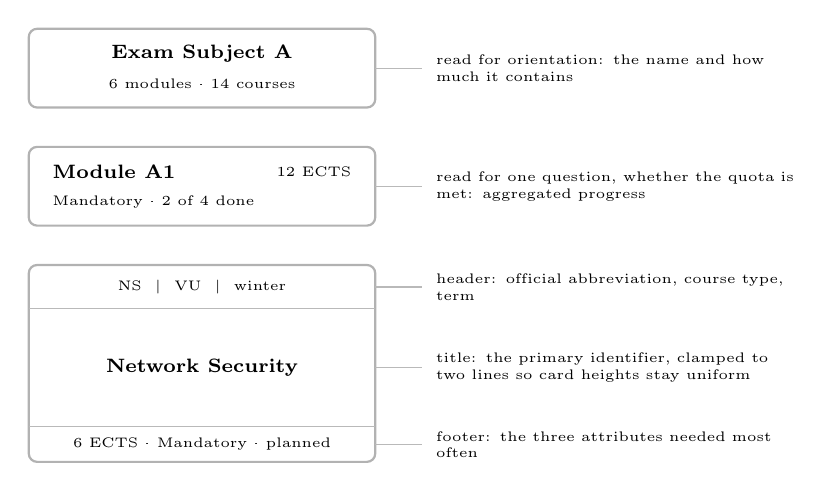
\begin{tikzpicture}[font=\scriptsize,
  ann/.style={font=\tiny, text=black, anchor=west, text width=4.6cm, align=left},
  tick/.style={gray!55, thin}]

  % --- Exam subject card ---
  \draw[gray!60, line width=0.8pt, rounded corners=3pt, fill=white] (0,0) rectangle (4.4,1.0);
  \node[font=\scriptsize\bfseries] at (2.2,0.68) {Exam Subject A};
  \node[font=\tiny] at (2.2,0.3) {6 modules \textperiodcentered\ 14 courses};
  \draw[tick] (4.4,0.5) -- (5.0,0.5);
  \node[ann] at (5.05,0.5) {read for orientation: the name and how much it contains};

  % --- Module header ---
  \draw[gray!60, line width=0.8pt, rounded corners=3pt, fill=white] (0,-1.5) rectangle (4.4,-0.5);
  \node[font=\scriptsize\bfseries, anchor=west] at (0.18,-0.82) {Module A1};
  \node[font=\tiny, anchor=east] at (4.22,-0.82) {12~ECTS};
  \node[font=\tiny, anchor=west] at (0.18,-1.2) {Mandatory \textperiodcentered\ 2 of 4 done};
  \draw[tick] (4.4,-1.0) -- (5.0,-1.0);
  \node[ann] at (5.05,-1.0) {read for one question, whether the quota is met: aggregated progress};

  % --- Course card, three fixed zones ---
  \draw[gray!60, line width=0.8pt, rounded corners=3pt, fill=white] (0,-4.5) rectangle (4.4,-2.0);
  \draw[tick] (0,-2.55) -- (4.4,-2.55);
  \draw[tick] (0,-4.05) -- (4.4,-4.05);
  \node[font=\tiny] at (2.2,-2.28) {NS \ $|$ \ VU \ $|$ \ winter};
  \node[font=\scriptsize\bfseries, text width=3.9cm, align=center] at (2.2,-3.3) {Network Security};
  \node[font=\tiny] at (2.2,-4.28) {6~ECTS \textperiodcentered\ Mandatory \textperiodcentered\ planned};

  \draw[tick] (4.4,-2.28) -- (5.0,-2.28);
  \node[ann] at (5.05,-2.28) {header: official abbreviation, course type, term};
  \draw[tick] (4.4,-3.3) -- (5.0,-3.3);
  \node[ann] at (5.05,-3.3) {title: the primary identifier, clamped to two lines so card heights stay uniform};
  \draw[tick] (4.4,-4.28) -- (5.0,-4.28);
  \node[ann] at (5.05,-4.28) {footer: the three attributes needed most often};
\end{tikzpicture}
\caption{Text carried at each hierarchy level. The exam-subject card states only extent, the module header aggregates progress, and the course card divides its text into three zones of fixed height.}
\label{fig:card-text}
\end{figure}


Three alternatives were weighed and rejected, each on the same trade between information and height: \emph{richer metadata on course cards} roughly doubles card height for information a routine placement does not need (T54); \emph{module headers reduced to name and ECTS} force an expand or a Dashboard visit to read progress; and \emph{a full course list in the module header} makes a collapsed module nearly as tall as an expanded one. 
% ------------------------------------------------------------

\section{Interaction Design}
\label{sec:interaction}
The subsections below proceed from the overall workflow a student follows, to the underlying state model that workflow operates on, to the general interaction principles (dual drag/button paths, context-sensitive actions) applied throughout, to the specific mechanisms (Semester Picker, popover, module interaction) built from those principles. Because these principles hold across both views, they are stated before the views themselves. Two surfaces they act on are therefore named here and designed later: a \emph{semester lane}, the column holding the courses assigned to one semester, and the \gterm{parking-stage}{Parking Stage}, the area beside those lanes holding courses saved but not yet assigned to a term (both Section~\ref{sec:table-view}).


\subsection{Planning Workflow}
\label{sec:workflow}

Students build their curricula in an exploration-first sequence. As one participant noted, finding interesting courses is \enquote{cool as a first step… not thinking yet about which semester} (T20). Students distinctly separate the act of exploring options from the act of committing them to a timeline, explicitly stating that the \enquote{graph used for exploration, not planning} (T20). 

To support this mental model and provide a guided onboarding experience (Feature~\ref{feat:006}, Req.~1), the interface introduces an intermediate staging area between discovery and semester assignment (Feature~\ref{feat:004}, Req.~2). Consequently, the tool is designed around a three-stage planning workflow (Figure~\ref{fig:workflow}):
\begin{enumerate}
  \item \textbf{Browse:} The student opens the Graph View or the Sidebar and explores the full curriculum using search, filters, and collapse controls to manage visual density.
  \item \textbf{Shortlist:} The student parks interesting courses into the Parking Stage without needing to commit them to a specific semester.
  \item \textbf{Assign:} The student switches to the Table View and drags parked courses into semester lanes, or uses the Semester Picker to assign them directly.
\end{enumerate}

This intended sequence is gently surfaced through the onboarding tooltip flow and the default-collapsed graph state, which encourages high-level exploration before commitment. Furthermore, the Parking Stage is positioned prominently at the top of every Semester Picker (Section~\ref{sec:semester-picker}) to bridge the gap between shortlisting and assigning. 

The workflow does not force staging for every decision. A student who already knows their plan can bypass the Shortlist step entirely, assigning a course directly to a semester using the context-sensitive Semester Picker (Section~\ref{sec:semester-picker}), as illustrated by the direct assignment path in Figure~\ref{fig:workflow}.

\begin{figure}[htbp]
\centering
\begin{tikzpicture}[font=\small, scale=0.88, transform shape]
  \def\bw{3.4}\def\bh{3.0}

  % Step 1: Browse
  \fill[subjectblue20, rounded corners=5pt] (0,0) rectangle (\bw,\bh);
  \draw[subjectblue!50, line width=0.8pt, rounded corners=5pt]
    (0,0) rectangle (\bw,\bh);
  \node[font=\footnotesize\bfseries] at (\bw/2, 2.6) {1 \quad Browse};
  \node[text width=2.9cm, align=center, font=\scriptsize]
    at (\bw/2, 1.6) {Explore the full curriculum in Graph View or Sidebar};
  \node[font=\tiny, text width=2.9cm, align=center]
    at (\bw/2, 0.35) {\textit{Graph View}};

  % Arrow 1 → 2
  \draw[-{Stealth[length=5pt]}, subjectblue!70, line width=1pt]
    (\bw+0.1, \bh/2) -- (\bw+0.6, \bh/2);

  % Step 2: Shortlist
  \def\ox{4.0}
  \fill[subjectgreen20, rounded corners=5pt] (\ox,0) rectangle (\ox+\bw,\bh);
  \draw[subjectgreen!50, line width=0.8pt, rounded corners=5pt]
    (\ox,0) rectangle (\ox+\bw,\bh);
  \node[font=\footnotesize\bfseries] at (\ox+\bw/2, 2.6) {2 \quad Shortlist};
  \node[text width=2.9cm, align=center, font=\scriptsize]
    at (\ox+\bw/2, 1.6) {Park interesting courses without committing to a semester};
  \node[font=\tiny, text width=2.9cm, align=center]
    at (\ox+\bw/2, 0.35) {\textit{Parking Stage}};

  % Arrow 2 → 3
  \draw[-{Stealth[length=5pt]}, subjectgreen!70, line width=1pt]
    (\ox+\bw+0.1, \bh/2) -- (\ox+\bw+0.6, \bh/2);

  % Step 3: Assign
  \def\ox{8.0}
  \fill[subjectorange20, rounded corners=5pt] (\ox,0) rectangle (\ox+\bw,\bh);
  \draw[subjectorange!50, line width=0.8pt, rounded corners=5pt]
    (\ox,0) rectangle (\ox+\bw,\bh);
  \node[font=\footnotesize\bfseries] at (\ox+\bw/2, 2.6) {3 \quad Assign};
  \node[text width=2.9cm, align=center, font=\scriptsize]
    at (\ox+\bw/2, 1.6) {Drag (parked) courses into semester lanes or use the Semester Picker};
  \node[font=\tiny, text width=2.9cm, align=center]
    at (\ox+\bw/2, 0.35) {\textit{Table View}};

  % Arrow 1 → 3 (Direct Assign Bypass)
  \draw[-{Stealth[length=5pt]}, gray!70, dashed, line width=1pt]
    (\bw/2, -0.1) to[out=-20, in=-160] node[below, font=\scriptsize, text=black] {Direct Assign} (8.0+\bw/2, -0.1);

\end{tikzpicture}
\caption{Three-stage planning workflow: Browse (Graph View), Shortlist (Parking Stage) and Assign (Table View, committing to a semester). The Shortlist stage can be bypassed and a course assigned directly.}
\label{fig:workflow}
\end{figure}

% ============================================================
\subsection{Course Lifecycle and State Machine}
\label{sec:lifecycle}

To support clear user comprehension, the interface requires a strict distinction between not-planned, planned, and completed courses, utilising consistent visual encodings across all views (Feature~\ref{feat:002}, Req.~4). Consequently, every course in the curriculum exists in exactly one of four lifecycle states at any given time: \emph{not planned}, \emph{parked}, \emph{planned}, or \emph{done} (Figure~\ref{fig:state-machine}).

\begin{figure}[htbp]
\centering
\begin{tikzpicture}[
  state/.style={draw=gray!60, rounded corners=5pt, minimum width=2.3cm,
                minimum height=0.75cm, align=center, font=\small, fill=gray!8},
  tr/.style={-{Stealth[length=4.5pt]}, gray!70, font=\scriptsize},
  lbl/.style={font=\scriptsize, text=black, fill=white, inner sep=1pt}
]
  % States
  \node[state] (NP)     at (0,0)    {Not Planned};
  \node[state] (PK)     at (0,-2.5) {Parked};
  \node[state] (PL)     at (5,0)    {Planned};
  \node[state] (DO)     at (5,-2.5) {Done};

  % Initial state marker
  \fill[black] (-1.8,0) circle (0.1);
  \draw[tr, black] (-1.7,0) -- (NP.west);

  % NP <-> Parked (Left Vertical)
  \draw[tr] ([xshift=0.15cm]NP.south) -- node[lbl, right] {Park} ([xshift=0.15cm]PK.north);
  \draw[tr] ([xshift=-0.15cm]PK.north) -- node[lbl, left] {Remove} ([xshift=-0.15cm]NP.south);

  % NP <-> Planned (Top Horizontal)
  \draw[tr] ([yshift=0.15cm]NP.east) -- node[lbl, above] {Add to plan} ([yshift=0.15cm]PL.west);
  \draw[tr] ([yshift=-0.15cm]PL.west) -- node[lbl, below] {Remove} ([yshift=-0.15cm]NP.east);

  % PL <-> Done (Right Vertical)
  \draw[tr] ([xshift=-0.15cm]PL.south) -- node[lbl, left] {Mark done} ([xshift=-0.15cm]DO.north);
  \draw[tr] ([xshift=0.15cm]DO.north) -- node[lbl, right] {Unmark} ([xshift=0.15cm]PL.south);

  % Parked <-> Planned (Diagonal). Two parallel arrows: a planned course can be
  % returned to the shortlist through the Semester Picker, not only removed.
  \draw[tr] ([yshift=0.16cm]PK.north east) -- node[lbl, above, sloped, pos=0.26] {Add to plan} ([yshift=0.16cm]PL.south west);
  \draw[tr] ([yshift=-0.16cm]PL.south west) -- node[lbl, below, sloped, pos=0.74] {Park} ([yshift=-0.16cm]PK.north east);

  % Done -> NP (Diagonal Up-Left)
  % Setting pos=0.2 keeps the label close to the 'Done' node (bottom right)
  \draw[tr] (DO.north west) -- node[lbl, above, sloped, pos=0.18] {Remove} (NP.south east);

\end{tikzpicture}
\caption{Course lifecycle state machine. Every course is in exactly one of four states at any time, and every transition the interface offers is drawn here.}
\label{fig:state-machine}
\end{figure}

The system enforces specific, user-triggered transitions between these states, shown together with the action buttons that trigger each transition in Figure~\ref{fig:action-buttons} below:
\begin{itemize}
  \item \textbf{Assign:} \emph{not planned} or \emph{parked} $\to$ \emph{planned} (assigning to a semester).
  \item \textbf{Park:} \emph{not planned} or \emph{planned} $\to$ \emph{parked} (shortlisting a course, or returning a planned one to the shortlist without discarding it).
  \item \textbf{Complete:} \emph{planned} $\leftrightarrow$ \emph{done} (marking or unmarking as completed).
  \item \textbf{Remove:} any state $\to$ \emph{not planned} (removing the course from the plan).
\end{itemize}
The return path from \emph{planned} to \emph{parked} needs no control of its own: moving a planned course opens the same Semester Picker, which lists the Parking Stage above the semesters (Section~\ref{sec:semester-picker}).

A \emph{free-form tag system} was rejected because the Compliance Engine needs a machine-readable planned-versus-done distinction to compute progress, which arbitrary user tags cannot supply; an intermediate \emph{in-progress} state was excluded because the tool works at semester granularity (OOS2).
\subsection{Drag-and-Drop and Button Interaction Paths}
\label{sec:interaction-paths}
Students expect both explicit button actions for planning and direct spatial manipulation, often asking to \enquote{drag and drop somehow} (T21, T44). Consequently, the design treats these not as mutually exclusive choices, but as complementary interaction paths (Feature~\ref{feat:004}). Providing a visible button-based equivalent for every drag action aligns with Nielsen's recognition-rather-than-recall heuristic~\cite{nielsen1994}. Visible buttons make available actions salient immediately, rather than forcing users to guess if a drag gesture is supported. This dual approach ensures accessibility for students unable to perform precise drag gestures (e.g., using a trackpad or with motor impairments) and supports workflows where dragging is impossible, such as adding a course directly from the Graph View. Furthermore, students require robust, data-safe replanning capabilities (Feature~\ref{feat:004}, Req.~3; Feature~\ref{feat:008}, Req.~1, Req.~4). By leveraging the shared planning-state model (Section~\ref{sec:canvas}), moving a planned course acts as a direct state update. Because the Compliance Engine (Section~\ref{sec:compliance}) recomputes dynamically after every action, rapid replanning becomes a natural, immediate consequence of these interaction paths.

To realise this, the interface provides two complementary mechanisms for every core action. Drag-and-drop serves as the primary mechanism for \emph{spatial repositioning}. Students can move a course card between the curriculum pool, a semester lane, and the Parking Stage, or freely reorder cards within a specific lane. In contrast, buttons serve as the primary mechanism for \emph{state transitions}, such as adding a course to the plan (which opens the Semester Picker detailed in Section~\ref{sec:semester-picker}), marking a course as completed, or removing it. These paths overlap. Dragging a parked course into a semester lane simultaneously performs a spatial move and a state transition to \emph{planned}. Additionally, dragging a card past the last visible semester lane automatically generates a new lane in place. This mirrors the progressive reveal of the button-triggered Semester Picker (Section~\ref{sec:semester-picker}), allowing students to extend their timeline without switching interaction contexts.

\emph{Drag-and-drop only} was rejected for the accessibility and discoverability reasons above, for its incompatibility with the Graph View, and because some participants preferred table-like interaction (T47); \emph{buttons only} was rejected because it removes the spatial rearrangement participants valued (T21, T28) and makes reordering a shortlist a sequence of menu clicks. 

% ------------------------------------------------------------
\subsection{Context-Sensitive Action Buttons}
\label{sec:action-buttons}

To support a visual-first, low-text design (Feature~\ref{feat:011}, Req.~1) and minimise visual clutter (Feature~\ref{feat:011}, Req.~4), only the actions valid for a course's \emph{current lifecycle state} are displayed on its card. Aligning with Nielsen's error prevention heuristic~\cite{nielsen1994}, invalid actions are omitted entirely rather than being displayed in a disabled or greyed-out state. This eliminates the cognitive overhead of parsing why a button is unavailable and keeps the action zone small, leaving the majority of the card surface dedicated to curriculum content. Depending on its current state, a card therefore displays only two to three buttons, as the state mappings in Figure~\ref{fig:action-buttons} show.

To prevent action affordances from being misread as status or compliance signals, the majority of buttons are rendered in a neutral grey, deliberately keeping them outside the curriculum's hue-based encoding system (Section~\ref{sec:subject-colour}). The sole exception is the \emph{Remove} button, which is rendered in red. Because red is intentionally excluded from the general subject-colour palette, its isolated use here unambiguously signals a destructive action, providing a clear visual warning before a course is deleted from the plan.

\begin{figure}[htbp]
\centering
\begin{tikzpicture}[
  font=\sffamily,
  statebox/.style={draw=gray!60, fill=gray!5, rounded corners=4pt, line width=0.8pt, minimum width=4.8cm, minimum height=1.6cm},
  btn/.style={draw=gray!50, fill=white, rounded corners=2pt, inner sep=2.5pt, font=\scriptsize},
  header/.style={font=\small\bfseries, text=black},
  tr/.style={-{Stealth[length=5pt]}, gray!80, line width=0.8pt},
  lbl/.style={font=\scriptsize, text=black, fill=white, inner sep=2pt}
]

  \def\xoff{8.2}
  \def\yoff{4.2}

  % --- Nodes ---
  
  % 1. Not Planned
  \node[statebox] (NP) at (0, \yoff) {};
  \node[header, anchor=north] at (NP.north) [yshift=-4pt] {Not Planned};
  \draw[gray!30, thin] ([yshift=-18pt]NP.north west) -- ([yshift=-18pt]NP.north east);
  \node[btn] at ([xshift=-1.1cm, yshift=12pt]NP.south) {Park};
  \node[btn] at ([xshift=1.1cm, yshift=12pt]NP.south) {Add to plan};

  % 2. Parked
  \node[statebox] (PK) at (0, 0) {};
  \node[header, anchor=north] at (PK.north) [yshift=-4pt] {Parked};
  \draw[gray!30, thin] ([yshift=-18pt]PK.north west) -- ([yshift=-18pt]PK.north east);
  \node[btn] at ([xshift=-1.1cm, yshift=12pt]PK.south) {Add to plan};
  \node[btn] at ([xshift=1.1cm, yshift=12pt]PK.south) {Remove};

  % 3. Planned
  \node[statebox] (PL) at (\xoff, \yoff) {};
  \node[header, anchor=north] at (PL.north) [yshift=-4pt] {Planned};
  \draw[gray!30, thin] ([yshift=-18pt]PL.north west) -- ([yshift=-18pt]PL.north east);
  \node[btn] at ([xshift=-1.6cm, yshift=12pt]PL.south) {Move};  % opens the Semester Picker, Parking Stage included
  \node[btn] at ([xshift=0cm, yshift=12pt]PL.south) {Mark done};
  \node[btn] at ([xshift=1.6cm, yshift=12pt]PL.south) {Remove};

  % 4. Done
  \node[statebox] (DO) at (\xoff, 0) {};
  \node[header, anchor=north] at (DO.north) [yshift=-4pt] {Done};
  \draw[gray!30, thin] ([yshift=-18pt]DO.north west) -- ([yshift=-18pt]DO.north east);
  \node[btn] at ([xshift=-1.1cm, yshift=12pt]DO.south) {Unmark};
  \node[btn] at ([xshift=1.1cm, yshift=12pt]DO.south) {Remove};

  % --- State Machine Transition Arrows ---

  % Initial state marker
  \fill[black] (-3.2, \yoff) circle (0.1);
  \draw[tr, black] (-3.1, \yoff) -- (NP.west);

  % NP <-> Parked (Left Vertical)
  \draw[tr] ([xshift=-0.5cm]NP.south) -- node[lbl, left] {Park} ([xshift=-0.5cm]PK.north);
  \draw[tr] ([xshift=0.5cm]PK.north) -- node[lbl, right] {Remove} ([xshift=0.5cm]NP.south);

  % NP <-> Planned (Top Horizontal)
  \draw[tr] ([yshift=0.25cm]NP.east) -- node[lbl, above] {Add to plan} ([yshift=0.25cm]PL.west);
  \draw[tr] ([yshift=-0.25cm]PL.west) -- node[lbl, below] {Remove} ([yshift=-0.25cm]NP.east);

  % PL <-> Done (Right Vertical)
  \draw[tr] ([xshift=0.5cm]PL.south) -- node[lbl, right] {Mark done} ([xshift=0.5cm]DO.north);
  \draw[tr] ([xshift=-0.5cm]DO.north) -- node[lbl, left] {Unmark} ([xshift=-0.5cm]PL.south);

  % Parked <-> Planned (Diagonal), mirroring the state machine above.
  \draw[tr] ([yshift=0.2cm]PK.north east) -- node[lbl, above, sloped, pos=0.27] {Add to plan} ([yshift=0.2cm]PL.south west);
  \draw[tr] ([yshift=-0.2cm]PL.south west) -- node[lbl, below, sloped, pos=0.73] {Park} ([yshift=-0.2cm]PK.north east);

  % Done -> NP (Diagonal Up-Left)
  \draw[tr] (DO.north west) -- node[lbl, above, sloped, pos=0.16] {Remove} (NP.south east);

\end{tikzpicture}
\caption{Unified course lifecycle state machine with context-sensitive action buttons. Each state strictly defines and displays only the active transitions available to the user.}
\label{fig:action-buttons}
\end{figure}

An \emph{overflow menu} was evaluated and rejected: it minimises chrome but puts the most frequent action, Add to plan, behind an extra click, which is a poor trade at the frequency these actions are used.

% ------------------------------------------------------------
\subsection{Semester Picker}
\label{sec:semester-picker}

To keep planning a course and selecting its target semester one interaction (Feature~\ref{feat:004}), the \gterm{semester-picker}{Semester Picker} appears as an inline menu anchored directly to the triggering card. This avoids interrupting the user's workflow with a separate screen and preserves their spatial context on the canvas. Reflecting the three-stage planning workflow (Section~\ref{sec:workflow}), the menu lists the \enquote{Parking Stage} at the top to support the shortlisting phase, followed by a chronological list of the student's planned semesters. 

To proactively prevent scheduling errors (Feature~\ref{feat:008}, Req.~3), this list is dynamically filtered based on the course's term availability. For example, a winter-only course displays only winter semesters as selectable options. To facilitate fluid long-term planning, the picker includes a progressive reveal design: it perpetually offers an option to assign the course to a new, future valid semester, extending the timeline organically without a separate configuration step.

Term availability filters the menu options strictly. The student's workload capacity is treated differently. That capacity is a per-semester credit and weekly-hour target held in the personal profile (Section~\ref{sec:profile}), and the picker only advises on it (OOS1): if a valid target semester would exceed it, the option remains selectable but carries a visually distinct warning. This design choice preserves the student's autonomy to intentionally exceed their planned workload based on their own judgement.
% ------------------------------------------------------------
\subsection{Notes, Hours, and Grade Popover}
\label{sec:popover}

A recurring request was to personalise the planning space. Participants asked a tool where they could \enquote{enter your grades and the hours} them (T12) while having \enquote{space to write something next to it} (T47). To support this, the system must retain user-owned planning fields (specifically notes, grades, and workload estimates) across data refreshes (Feature~\ref{feat:001}, Req.~4) and allow inline note-taking per course (Feature~\ref{feat:004}, Req.~5).

To achieve this without breaking the spatial context of the canvas, tapping the info icon on a course card opens an inline popover anchored directly to the card. The surrounding cards remain visible, and the canvas position is not altered. The popover contains three user-owned fields: a free-text notes field, a numeric estimated hours per week field, and a grade field. 

To prevent semantically invalid data entry, the grade field is strictly gated by the course lifecycle (Section~\ref{sec:lifecycle}). Because a grade inherently implies a final examination result, the field becomes editable only when a course is marked as \emph{done}; it remains locked in all other states. Furthermore, if a completed course is ever removed from the plan, its associated grade is automatically cleared. 

Alternative editing interfaces were considered but rejected. \emph{Inline editing directly on the card surface} was rejected because cards must maintain fixed dimensions for the table and graph geometry; a variable-height editing area would break positional consistency.

% ------------------------------------------------------------
\subsection{Module Interaction}
\label{sec:module-interaction}

Many students treat multi-course Master's modules as atomic units, preferring to add the entire module to their plan at once rather than course by course (T44, Feature~\ref{feat:004}). Students also requested clear visibility of their progress at the module level (T57, Feature~\ref{feat:002}). Furthermore, when interacting with these modules in the Graph View, collapsing a module must not trigger a layout reflow; maintaining stable node positions is essential to preserve the user's spatial memory of the curriculum map (Feature~\ref{feat:013}, Req.~2).

To support these workflows, module panels offer three specific interactions beyond individual course controls:
\begin{itemize}
  \item \textbf{Add entire module:} Assigns all member courses to a target semester in a single interaction.
  \item \textbf{Mark module done:} Flags all member courses as complete in one step.
  \item \textbf{Collapse/expand (Graph View):} Hides or reveals the module's member courses. When collapsed, the panel body is replaced by a structural placeholder of identical dimensions (e.g., a dashed-border outline), ensuring the module retains its exact footprint and prevents surrounding elements from shifting.
\end{itemize}

When a student manually adds a single course that belongs to a multi-course module, the system presents a confirmation prompt offering to add the entire module instead. This provides a shortcut for atomic modules while preventing accidental bulk additions for modules that contain mutually exclusive course options. Additionally, an aggregated status indicator in the module header provides the requested module-level progress overview.

\emph{Strictly course-by-course addition} adds friction to the common atomic-module case, and \emph{silent full-module addition} would add unwanted variants in modules with substitutable courses; the prompt is the middle path.


% ------------------------------------------------------------

\section{Visual Legend Design}
\label{sec:legend}
Feature~\ref{feat:010} documents that the visual encodings are not self-evident on first exposure: participants asked \enquote{what do these stand for?} (T41) and reported that shorthand labels are \enquote{not intuitively understandable} (T40). Feature~\ref{feat:010}, Req.~1 requires an always-available legend explaining symbols, colours, and status encodings. This is a second, more targeted realisation of the same \enquote{clearly comprehensive content} principle (Bartel et al.~\cite{bartel_design_2024}) that the first-use tooltip sequence addresses more generally (Section~\ref{sec:onboarding}); the paper's specific recommendation of a \enquote{help bar (context-sensitive help)} describes almost exactly a togglable, on-demand legend rather than a one-off tutorial a student sees once and cannot return to.

Based on this, a togglable legend panel, opened from a toolbar control and closable on demand, restates every visual encoding established elsewhere in this chapter in one place: the four planning-status states (Section~\ref{sec:status}), the subject-colour hierarchy (Section~\ref{sec:subject-colour}), and the obligation-type border encoding (Section~\ref{sec:obligation}). The legend is presented as sample cards rendered with the actual interface's own styling, rather than a text description, keeping it visually consistent with what it explains and avoiding a separate description that would need to stay synchronised with the encoding whenever it changes.


% ============================================================
\section{Graph View Design}
\label{sec:graph-spatial}
The Graph View provides a structured, network-based environment for exploring the curriculum. While the underlying concept of a graph-based view was established in the formative prototype (Chapter~\ref{chap:formative-study}), subsequent design efforts focused on refining its spatial hierarchy, node customisability, density management, and filtering mechanisms.

% ------------------------------------------------------------
\subsection{Left-to-Right Hierarchical Layout}
\label{sec:graph-ltr}
To align with natural reading habits in Western contexts, participants suggested a horizontal layout, noting it is \enquote{nicer if it goes left to right, because we read left to right} (Feature~\ref{feat:010}, T32). This direction maps increasing depth to increasing specificity while answering participants' questions about spatial meaning (\enquote{Is there any meaning to the vertical position?}, T27).

Based on this, the curriculum tree renders left-to-right across four depth levels (Programme $\to$ Exam Subject $\to$ Module $\to$ Course; Figure~\ref{fig:graph-schema}). Exam subjects are stacked as distinct horizontal bands on the vertical axis, fulfilling Feature~\ref{feat:010}, Req.~2's \emph{structured layout mode} and directly answering T27: vertical band membership explicitly encodes the exam subject. Two alternatives were weighed against this. The Figma prototype's \emph{radial layout} (Section~\ref{sec:prototype-elicitation}) placed the programme at the centre with subjects radiating outward; it was re-derived and replaced because depth is then encoded as distance from a centre rather than as reading direction, which is what T32 asked for, and because a radial arrangement leaves no free axis on which subject membership could be encoded. A \emph{force-directed layout} was rejected because node positions would be recomputed whenever the graph is expanded or filtered, which would destroy the spatial memory Feature~\ref{feat:013}, Req.~2 requires the layout to preserve.

\begin{figure}[htbp]
\centering
\begin{tikzpicture}[font=\scriptsize]
  % Subject band colours (very light fills)
  \fill[subjectblue!8]   (2.2,0) rectangle (11.0,2.8);
  \fill[subjectgreen!8]  (2.2,2.8) rectangle (11.0,5.2);
  \fill[subjectorange!8] (2.2,5.2) rectangle (11.0,7.2);

  % Column separators (dashed)
  \foreach \x in {2.2, 4.5, 7.5} {
    \draw[gray!25, dashed, line width=0.5pt] (\x,0) -- (\x,7.2);
  }
  \draw[gray!25, dashed, line width=0.5pt] (11.0,0) -- (11.0,7.2);

  % Column headers
  \node[font=\tiny] at (3.3,7.5)  {Exam Subject};
  \node[font=\tiny] at (6.0,7.5)  {Module};
  \node[font=\tiny] at (9.2,7.5)  {Course};

  % Axis labels
  \draw[-{Stealth[length=4pt]}, gray!50] (2.2,-0.5) -- (11.2,-0.5);
  \node[font=\tiny] at (6.7,-0.85)
    {$\longrightarrow$ Curriculum depth (left to right)};

  \draw[-{Stealth[length=4pt]}, gray!50] (-0.5,0) -- (-0.5,7.5);
  \node[rotate=90, font=\tiny] at (-0.85,3.6)
    {$\longrightarrow$ Exam Subject band (vertical)};

  % Programme node
  \fill[gray!20, rounded corners=2pt] (0.1,3.35) rectangle (1.9,3.85);
  \draw[gray!50, rounded corners=2pt] (0.1,3.35) rectangle (1.9,3.85);
  \node[font=\tiny] at (1.0,3.6) {Programme};

  % Subject nodes
  \fill[subjectblue, rounded corners=2pt] (2.4,1.1) rectangle (4.3,1.6);
  \node[font=\tiny, text=white] at (3.35,1.35) {Sub. A};

  \fill[subjectgreen, rounded corners=2pt] (2.4,3.365) rectangle (4.3,3.865);
  \node[font=\tiny, text=white] at (3.35,3.615) {Sub. B};

  \fill[subjectorange, rounded corners=2pt] (2.4,6.0) rectangle (4.3,6.5);
  \node[font=\tiny, text=white] at (3.35,6.25) {Sub. C};

  % Edges: prog → subjects
  \draw[-{Stealth[length=3pt]},gray!50,thin] (1.9,3.6) -- (2.4,1.35);
  \draw[-{Stealth[length=3pt]},gray!50,thin] (1.9,3.6) -- (2.4,3.615);
  \draw[-{Stealth[length=3pt]},gray!50,thin] (1.9,3.6) -- (2.4,6.25);

  % Module nodes (Subject A)
  \fill[subjectblue20, rounded corners=2pt] (4.7,0.4) rectangle (7.1,0.85);
  \draw[subjectblue, line width=0.8pt, rounded corners=2pt] (4.7,0.4) rectangle (7.1,0.85);
  \node[font=\tiny] at (5.9,0.625) {Module A1};

  \fill[subjectblue20, rounded corners=2pt] (4.7,1.5) rectangle (7.1,1.95);
  \draw[subjectblue, line width=0.8pt, rounded corners=2pt] (4.7,1.5) rectangle (7.1,1.95);
  \node[font=\tiny] at (5.9,1.725) {Module A2};

  % Module node (Subject B)
  \fill[subjectgreen20, rounded corners=2pt] (4.7,3.065) rectangle (7.1,3.515);
  \draw[subjectgreen, line width=0.8pt, rounded corners=2pt] (4.7,3.065) rectangle (7.1,3.515);
  \node[font=\tiny] at (5.9,3.29) {Module B1};

  \fill[subjectgreen20, rounded corners=2pt] (4.7,4.065) rectangle (7.1,4.515);
  \draw[subjectgreen, line width=0.8pt, rounded corners=2pt] (4.7,4.065) rectangle (7.1,4.515);
  \node[font=\tiny] at (5.9,4.29) {Module B2};

  % Module node (Subject C)
  \fill[subjectorange20, rounded corners=2pt] (4.7,5.8) rectangle (7.1,6.25);
  \draw[subjectorange, line width=0.8pt, rounded corners=2pt] (4.7,5.8) rectangle (7.1,6.25);
  \node[font=\tiny] at (5.9,6.025) {Module C1};

  % Edges: subjects → modules
  \draw[-{Stealth[length=3pt]},gray!45,thin] (4.3,1.35) -- (4.7,0.625);
  \draw[-{Stealth[length=3pt]},gray!45,thin] (4.3,1.35) -- (4.7,1.725);
  \draw[-{Stealth[length=3pt]},gray!45,thin] (4.3,3.615) -- (4.7,3.29);
  \draw[-{Stealth[length=3pt]},gray!45,thin] (4.3,3.615) -- (4.7,4.29);
  \draw[-{Stealth[length=3pt]},gray!45,thin] (4.3,6.25) -- (4.7,6.025);

  % Course nodes (abbreviated), coloured border matches parent subject
  \foreach \y in {0.3, 0.85, 1.5, 1.95} {
    \fill[white, rounded corners=1.5pt] (7.4,\y) rectangle (10.7,\y+0.42);
    \draw[subjectblue, line width=0.8pt, rounded corners=1.5pt] (7.4,\y) rectangle (10.7,\y+0.42);
    \node[font=\tiny] at (9.05,\y+0.21) {Course};
  }
  \foreach \y in {3.065, 3.565, 4.065, 4.515} {
    \fill[white, rounded corners=1.5pt] (7.4,\y) rectangle (10.7,\y+0.42);
    \draw[subjectgreen, line width=0.8pt, rounded corners=1.5pt] (7.4,\y) rectangle (10.7,\y+0.42);
    \node[font=\tiny] at (9.05,\y+0.21) {Course};
  }
  \foreach \y in {5.8, 6.3} {
    \fill[white, rounded corners=1.5pt] (7.4,\y) rectangle (10.7,\y+0.42);
    \draw[subjectorange, line width=0.8pt, rounded corners=1.5pt] (7.4,\y) rectangle (10.7,\y+0.42);
    \node[font=\tiny] at (9.05,\y+0.21) {Course};
  }

  % Edges: modules → courses (simplified)
  \draw[-{Stealth[length=3pt]},gray!40,thin] (7.1,0.625) -- (7.4,0.51);
  \draw[-{Stealth[length=3pt]},gray!40,thin] (7.1,0.625) -- (7.4,1.06);
  \draw[-{Stealth[length=3pt]},gray!40,thin] (7.1,1.725) -- (7.4,1.71);
  \draw[-{Stealth[length=3pt]},gray!40,thin] (7.1,1.725) -- (7.4,2.16);
  \draw[-{Stealth[length=3pt]},gray!40,thin] (7.1,3.29) -- (7.4,3.275);
  \draw[-{Stealth[length=3pt]},gray!40,thin] (7.1,3.29) -- (7.4,3.775);
  \draw[-{Stealth[length=3pt]},gray!40,thin] (7.1,4.29) -- (7.4,4.275);
  \draw[-{Stealth[length=3pt]},gray!40,thin] (7.1,4.29) -- (7.4,4.725);
  \draw[-{Stealth[length=3pt]},gray!40,thin] (7.1,6.025) -- (7.4,6.01);
  \draw[-{Stealth[length=3pt]},gray!40,thin] (7.1,6.025) -- (7.4,6.51);
\end{tikzpicture}
\caption{Graph View spatial encoding schema. The horizontal axis encodes curriculum depth; the vertical axis encodes exam subject membership through horizontal bands.}
\label{fig:graph-schema}
\end{figure}

% ------------------------------------------------------------
\subsection{Personal Customisability of Node Positions}
\label{sec:card-ordering}

Bartel et al.'s~\cite{bartel_design_2024} combined principle of user-centred design and study-programme-specific personalisation advocates giving students active control over their planning environment. Motivated by this theoretical foundation and direct user feedback (T28: \enquote{place items how I want}), the system allows students to override the default algorithmic layout. This is formalised in Feature~\ref{feat:010}, Req.~2, which specifies both a structured and a free layout mode, and Feature~\ref{feat:013}, Req.~2, which requires these custom spatial arrangements to persist.

To satisfy these requirements while protecting the vertical subject-band structure established in Section~\ref{sec:graph-ltr}, customisability is deliberately restricted to the horizontal axis. A student may drag any node left or right within its column, and the resulting offset persists across sessions, fulfilling the free layout mode. The vertical axis remains managed by the system to prevent layout corruption, keeping subject bands intact. 

\emph{Full two-dimensional free layout} was tested during development but rejected because any vertical reordering would inevitably break the hierarchical subject-band structure over time, corrupting the layout whenever new subjects were expanded without any automatic way to re-resolve it.

% ------------------------------------------------------------
\subsection{Density Control and Multi-Dimensional Filtering}
\label{sec:collapse-and-filters}

A fully expanded 120-ECTS Master programme contains well over 100 nodes simultaneously, which overwhelms orientation before a student knows the layout (Feature~\ref{feat:009}, T50: \enquote{with graphs it kind of explodes}). Furthermore, students need to filter this content without losing context or deleting selections (Feature~\ref{feat:009}, Req.~1--3, T42).

To address density, each exam subject and module node is individually collapsible. The default state on first load is fully collapsed to the exam-subject level to allow exploration. Collapse state persists across sessions; when collapsed, the module body is replaced by a structural placeholder of identical dimensions to prevent layout reflow. Three batch presets (\emph{Collapse all}, \emph{Expand all}, and \emph{Restore my layout}) provide single-action control over overall density.

To complement structural folding, graph filtering operates as a purely visual, reversible layer that never alters planning data. It spans six independent dimensions: obligation type, ECTS range, course type, exam subject, planning status, and term availability. The two ways of combining them differ deliberately. Within one dimension, several selected values combine disjunctively, so a student can ask for \enquote{mandatory or constrained elective} in a single pass rather than one obligation category at a time. Across dimensions they combine conjunctively: a node stays visible only while it satisfies every active dimension, so one filter is enough to hide it however well it matches the others.
The two controls are kept from working against each other. When a student expands a node whose children the active filters would all hide, those filters are lifted for that node, so expanding never opens an empty container; and changing a filter never resets the graph's collapse state (Feature~\ref{feat:009}, Req.~2). Filter configurations persist across sessions as stable planning preferences.

A \emph{default-expanded layout} was rejected for the overload it produces on first load, and \emph{destructive filtering}, in which a filter removes non-matching courses from the plan rather than from view, because filtering must be a safe and reversible exploration tool; discarding selections would penalise exploration.


% ------------------------------------------------------------
\section{Table View Design}
\label{sec:table-view}

The Table View translates study planning into a shared spatial canvas designed for allocating, ordering, and comparing courses over time. Participants worked with the prototype's version of this view without objecting to its structure (Chapter~\ref{chap:formative-study}), so the design work below concerns its interactions, components and data presentation rather than the arrangement itself. 
% ------------------------------------------------------------
\subsection{Spatial Model of the Table View}
\label{sec:table-spatial}
Participants preferred a table at this stage, \enquote{I simply find it easier with tables} (T47), and worked with the prototype's column-per-semester arrangement without objecting to it (Chapter~\ref{chap:formative-study}, Section~\ref{sec:prototype-elicitation}). Representing semesters as vertical columns maps naturally onto a left-to-right reading direction and reinforces the concept of laying out a study plan chronologically (T21). Feature~\ref{feat:004}, Req.~6 further requires manual ordering and at least one automatic ordering mode, which presupposes a spatial model in which position remains meaningful and stable. Bartel et al.~\cite{bartel_design_2024} user-centred design and study-programme-specific personalisation principle motivates keeping the vertical axis free for the student's own ordering rather than a system-imposed one, consistent with the same customisability argument used for card ordering elsewhere in this chapter (Section~\ref{sec:card-ordering}). Fixed lane widths are also necessary for the snap-grid system and for visual comparison across adjacent semesters: irregular columns would weaken alignment and make course distribution harder to assess at a glance.

% ------------------------------------------------------------
\subsection{Semester Lanes and Header Information}
\label{sec:semester-lanes}

Semester overload is noticed only once a semester is already loaded (Feature~\ref{feat:005}; T35, T4), so the load signal has to sit exactly where course-allocation decisions are made. Participants also asked for \enquote{space to write something next to it} (Feature~\ref{feat:004}, T47). Bartel et al.~\cite{bartel_design_2024} \enquote{clear presentation of curriculum information} principle explicitly recommends that \enquote{course names (including module affiliation)} and similar decision-relevant attributes be \enquote{displayed directly} rather than requiring a further click, from which the ECTS total in the lane header follows.

Based on this, the lane header displays the semester label, winter or summer semester and year (e.g., \enquote{WS 2025/26}) together with a continuously updated ECTS total, following progressive disclosure: ECTS load is permanently visible because it is needed continuously, whereas secondary indicators, estimated hours per week, ECTS-weighted mean grade, per-course notes, and a free-text semester note field, are available on demand through an on-demand popover rather than turning the lane header into a visually dense control area. A student can choose between two automatic sort modes, alphabetical or by ECTS weight, applied within each lane, while allowing users to return to their manual arrangement afterwards.

\emph{Showing semester totals only in the Dashboard} was rejected because the Dashboard is a separate overview component and does not provide immediate feedback during course placement. \emph{Keeping all semester statistics permanently visible} was rejected because it would increase background clutter during active planning, even though these details are only intermittently needed.

\subsection{Parking Stage}
\label{sec:parking}
The Shortlist stage of the planning workflow (Section~\ref{sec:workflow}) needs a place on the canvas, described by participants as \enquote{pool… with the courses… where I can move them around} (T21). It is realised as a Parking Stage positioned directly to the left of the active semester lanes. To visually separate it from active planning, the Parking Stage intentionally omits chronological and workload indicators, acting purely as a holding area. Because it shares the same continuous canvas as the semester lanes, students can evaluate parked courses alongside their committed schedule and drag one into a target semester while deciding, e.g.\ whether a course belongs in Semester 3 or Semester 4. If a student needs to focus exclusively on their active timeline without distractions, this staging area can be collapsed to reduce visual noise.

An alternative staging layout was considered but rejected. \emph{Representing parked courses as a disconnected sidebar list} was rejected because it breaks the spatial mapping of the course lifecycle (Section~\ref{sec:lifecycle}). Since \emph{parked} is an intermediate state between \emph{not planned} and \emph{planned}, its physical location must reflect this progression. Placing the Parking Stage directly on the canvas between the search sidebar (\emph{not planned}) and the semester lanes (\emph{planned}) creates a logical, left-to-right pipeline. Forcing parked courses back into a sidebar would visually regress them to the exploration phase and disrupt fluid drag-and-drop comparisons.

\subsection{Module Backgrounds}
\label{sec:modules-in-table}
To support per-module progress tracking (Feature~\ref{feat:002}, T57) and maintain consistent item identity across views (Feature~\ref{feat:004}), multi-course modules are represented as grouped visual containers. In the Table View, such a module renders as a soft background panel wrapping its member course cards, tinted with the shared subject colour (Section~\ref{sec:subject-colour}). Because vertical ordering within a lane is fully flexible, meaning a module's member courses do not need to be adjacent and can span different semesters, a permanently fixed panel would distort the layout or restrict placement. Instead, the background panel appears dynamically only when a member card is hovered, clicked, or dragged. Single-course modules bypass this panel treatment, collapsing directly into standard course cards (Section~\ref{sec:curriculum-abstraction}).

\emph{Custom-shaped connectors} bridging separated member cards were rejected as they introduce high structural complexity for minimal functional gain over the interaction-triggered panel.

% ============================================================
\section{Sidebar Design}
\label{sec:sidebar-design}
The searchable Course Catalogue sidebar is carried over directly from the prototype (Section~\ref{sec:prototype-elicitation}), where six participant walkthroughs raised no objection to it, so it is recorded here rather than re-derived. It occupies the left panel in the Table View (Section~\ref{sec:three-panels}) and lists the whole curriculum grouped by exam subject, with modules collapsible beneath their subject. A free-text field searches course and module names as well as the official course codes, and a course or a whole multi-course module is dragged from the list straight into a semester lane, or added through the Semester Picker (Section~\ref{sec:interaction-paths}). Nothing in it was changed in response to the formative interviews, and no participant asked for it to be different.

% ============================================================
\section{Onboarding and First-Use Design}
\label{sec:onboarding}
The sections above describe a tool in use. This one describes the state it starts in, before the student has a plan or a configured programme. The transition to self-managed study planning was described as a \enquote{shock} (T59) and as \enquote{one of the most difficult things for first-years} (T59). Starting with an empty and unconfigured canvas would likely intensify this problem: without basic programme information, the system cannot display meaningful ECTS targets, semester labels, or compliance rules, which may make the tool seem unclear or incomplete. Feature~\ref{feat:006}, Req.~2 further records that planning needs differ between early-stage students, who mainly follow mandatory courses, and later-stage students, who make more individual choices. Bartel et al.~\cite{bartel_design_2024} \enquote{clearly comprehensive content} principle recommends specifically \enquote{a tool guide for first-time use}, on the grounds that a digital study assistant is a novel type of application for most students and cannot assume prior familiarity; the tooltip sequence below is the direct realisation of that recommendation.

Based on this, a programme setup dialog is shown on first login, before the student reaches the canvas. It collects the degree programme and the start semester (season and year), the minimum needed to configure ECTS targets, compliance rules, semester labels, and term-availability constraints. After setup, an empty plan triggers a pre-fill offer: the student may accept a template plan based on a standard first-attempt schedule for the selected programme, or decline and build from scratch (Feature~\ref{feat:001}, Req.~5). A lightweight tooltip sequence is shown on first visit to each major view, guiding the student through the workflow (Feature~\ref{feat:006}, Req.~1). The setup dialog establishes the necessary context from the outset, while the optional pre-fill plan addresses the cold-start problem by offering an initial orientation without constraining students who prefer to plan independently.

% ============================================================
\section{Compliance Engine Design}
\label{sec:compliance}
Manual compliance checking was described as effortful and unreliable: Feature~\ref{feat:003}, T13: \enquote{Excel doesn't know your requirements… you have to double and triple check everything}. Bartel et al.~\cite{bartel_design_2024} \enquote{\emph{support during planning difficulties}} principle calls specifically for design that contributes to avoiding planning errors and for \enquote{clearly recognisable warnings and hints in case of planning obstacles}, which real-time, automatic checking directly provides. Feature~\ref{feat:003}, Req.~1 (real-time fulfilment update), Req.~2 (hard rules blocking), Req.~3 (soft warnings non-blocking), Req.~4 (missing list updated in real time), and Req.~5 (compliance shared across views) together call for a single authoritative check invoked on every change, and institutional rules changing between academic years calls for that check to live somewhere updatable without an application release.

Based on this, a dedicated rule engine is invoked after every frontend planning action (course added, moved, removed; status toggled, etc.), returning the resulting overall status, per-category ECTS statistics, a list of hard violations (unmet prerequisites or quota breaches), and a list of soft advisory warnings (recommended sequencing observations). Hard violations are surfaced as persistent, non-dismissible notifications; soft warnings as dismissible Dashboard notices; both update in real time, removing the compliance-checking loop from user memory. Judel et al.~\cite{judel_supporting_2023} describe an almost identical hard/soft distinction in a closely related study-planning tool, recommendations versus requirements, with each surfaced through distinct visual indicators rather than one undifferentiated warning; the Compliance Engine's separate treatments follow the same distinction.

Bartel et al.'s call for \emph{clearly recognisable} warnings within the same \enquote{\emph{support during planning difficulties}} guideline requires feedback to be immediately intelligible: if a student has to pause and deduce which of their recent actions triggered a violation, the burden the automatic check was meant to remove has been shifted rather than resolved. Compliance messages are therefore constructed to name the specific course, semester and action that triggered them. Rather than reporting a category of violation, the engine uses the same underlying rule to produce a situation-specific message according to whether a course was just added, moved, or altered; generic static strings would force students to reconstruct their own interaction history, especially after several rapid adjustments.

% ============================================================
\section{Dashboard Design}
\label{sec:dashboard}

The Dashboard is the right panel of the three-panel shell (Section~\ref{sec:three-panels}) and the interface realisation of Feature~\ref{feat:002}. Students conceptualise their progress at multiple granularities (current semester, upcoming semesters, and the overall programme; T1) and require an always-current, ambient placement to constantly answer, \enquote{where am I right now?} (T16). Furthermore, they explicitly want to separate what they have merely chosen from what they have already completed (T19). 

To address this, the Dashboard aggregates multiple progress indicators into a unified visual display~\cite{schwendimann2017}. Wienand et al.~\cite{wienand_design_2024} report the same concern from the other side: having made their own courses more flexible, they anticipated that students \enquote{might feel lost on how much progress they already made}, and answered it with progress bars at three nested levels, the chapter, the sub-chapter, and the whole course. Following that pattern, the Dashboard expands the student's mental model into four distinct, decision-relevant granularities (Figure~\ref{fig:dashboard-levels}):

\begin{enumerate}
  \item \textbf{Programme level:} Total ECTS planned and done versus required, overall completion percentage, and a major requirement checklist.
  \item \textbf{Category level:} ECTS breakdowns by obligation category (mandatory, constrained elective, fully elective, transferable skills) and by exam subject.
  \item \textbf{Semester level:} Per-semester ECTS bars showing planned and completed credits separately.
  \item \textbf{Module level:} Per-module progress bars.
\end{enumerate}

Aligning with Bartel et al.~\cite{bartel_design_2024} principles of user-centred personalisation, these sections are not locked into a fixed order. Each level is individually collapsible and freely reorderable, allowing students to hide irrelevant metrics and surface the granularities they need most. To provide positive reinforcement (Feature~\ref{feat:011}, Req.~3), which Wienand et al.~\cite{wienand_design_2024} likewise carry as a design principle for motivational elements, transient milestone notifications fire when overall completion reaches 25\,\%, 50\,\%, 75\,\%, and 100\,\%.

To satisfy the need to separate planned intent from actual completion (T19), the Dashboard features two top-level modes: \emph{Planning mode} (planned plus done) and \emph{Done mode} (done only). The collapse states and section orders are tracked independently for each mode. A student can keep the Semester level expanded on top while looking ahead in Planning mode, but configure the Module level to sit on top when reviewing historical progress in Done mode.

In addition to visualising current and historical data, the Dashboard functions as a real-time simulation tool that respects individual pacing preferences (T18). Aligning with Bartel et al.'s~\cite{bartel_design_2024} call for systems to account for planned semester workloads, the Semester-level progress bars dynamically evaluate the student's planned ECTS for each term against their recommended pacing target, which is read directly from their existing capacity profile (Section~\ref{sec:profile}). A student therefore sees an over- or under-loaded semester against their own capacity without entering that capacity a second time.

Feature~\ref{feat:002}, Req.~6 mandates that a student must immediately observe the effect of adding or removing a course on their progress and completion projection. Because the Dashboard and Compliance Engine (Section~\ref{sec:compliance}) operate in real time, every planning action instantly recomputes ECTS totals, category breakdowns, and pacing projections. Consequently, a student can simulate \enquote{what happens if I add this course} by dropping it onto the canvas, and undo the simulation just as easily by removing it. This leverages the established one-action interaction paths (Section~\ref{sec:interaction-paths}) without forcing the user into a separate, explicitly \enquote{tentative} preview mode.

Four alternatives were rejected. A \emph{single-level ECTS bar} hides category deficiencies behind a healthy total. A \emph{separate Dashboard screen} breaks the ambient, at-a-glance orientation T16 asks for. A \emph{shared section order across both modes} ignores that planning forward and reviewing back are different tasks. And a \emph{dedicated preview mode} would duplicate the shared state model (Section~\ref{sec:canvas}) when dropping a card onto the canvas already simulates the change.
\begin{figure}[htbp]
\centering
\begin{tikzpicture}[font=\scriptsize, scale=0.9, transform shape]
  \def\pw{4.2}

  % Programme level
  \fill[panelgray, rounded corners=4pt] (0,7.6) rectangle (\pw,8.6);
  \node[font=\scriptsize\bfseries, anchor=west] at (0.15,8.3) {Programme};
  \fill[gray!15, rounded corners=2pt] (0.15,7.85) rectangle (\pw-0.15,8.1);
  \fill[subjectblue, rounded corners=2pt] (0.15,7.85) rectangle (0.15+2.4,8.1);
  \node[font=\tiny, anchor=west] at (0.15,7.72) {67\,\% complete};

  % Category level
  \fill[panelgray, rounded corners=4pt] (0,6.1) rectangle (\pw,7.4);
  \node[font=\scriptsize\bfseries, anchor=west] at (0.15,7.1) {Category};
  \foreach \y/\frac/\col in {6.8/0.9/subjectblue, 6.55/0.5/subjectgreen, 6.3/0.3/subjectorange} {
    \fill[gray!15, rounded corners=1pt] (0.15,\y) rectangle (\pw-0.15,\y+0.16);
    \pgfmathsetmacro{\barlen}{(\pw-0.3)*\frac}
    \fill[\col, rounded corners=1pt] (0.15,\y) rectangle (0.15+\barlen,\y+0.16);
  }

  % Semester level
  \fill[panelgray, rounded corners=4pt] (0,4.4) rectangle (\pw,5.9);
  \node[font=\scriptsize\bfseries, anchor=west] at (0.15,5.6) {Semester};
  \foreach \y/\frac in {5.3/0.8, 5.05/0.6, 4.8/0.4, 4.55/0.15} {
    \fill[gray!15, rounded corners=1pt] (0.15,\y) rectangle (\pw-0.15,\y+0.16);
    \pgfmathsetmacro{\barlen}{(\pw-0.3)*\frac}
    \fill[plannedfill, rounded corners=1pt] (0.15,\y) rectangle (0.15+\barlen,\y+0.16);
    \draw[gray!50, rounded corners=1pt, line width=0.4pt] (0.15,\y) rectangle (0.15+\barlen,\y+0.16);
  }

  % Module level
  \fill[panelgray, rounded corners=4pt] (0,2.5) rectangle (\pw,4.2);
  \node[font=\scriptsize\bfseries, anchor=west] at (0.15,3.9) {Module};
  \foreach \y/\frac in {3.6/1.0, 3.35/0.7, 3.1/0.45, 2.85/0.2, 2.6/0.05} {
    \fill[gray!15, rounded corners=1pt] (0.15,\y) rectangle (\pw-0.15,\y+0.14);
    \pgfmathsetmacro{\barlen}{(\pw-0.3)*\frac}
    \fill[subjectgreen20, rounded corners=1pt] (0.15,\y) rectangle (0.15+\barlen,\y+0.14);
    \draw[subjectgreen, rounded corners=1pt, line width=0.4pt] (0.15,\y) rectangle (0.15+\barlen,\y+0.14);
  }

  % collapse chevrons (indicating each level is individually collapsible)
  \foreach \y in {8.3, 7.1, 5.6, 3.9} {
    \node[font=\tiny] at (\pw-0.28,\y) {$\vee$};
  }

\end{tikzpicture}
\caption{The Dashboard's four aggregation levels: Programme, Category, Semester, and Module. Each section collapses independently and the overall order is student-configurable.}
\label{fig:dashboard-levels}
\end{figure}

% ============================================================
\section{Profile Design}
\label{sec:profile}
Unintentional semester overload was reported repeatedly (T20, T35), alongside a need for workload limits set per student (T4). To address this (Feature~\ref{feat:005}, Req.~1--2) and to gather explicit inputs for the recommendation engine (Section~\ref{sec:rec-types-evidence}), each student maintains a central, configurable personal profile. This profile governs two distinct domains: workload capacity and recommendation personalisation. It is deliberately not part of the first-use setup dialog, which collects only what the system cannot start without (Section~\ref{sec:onboarding}); the profile is reachable from the toolbar at any point and every field in it can be changed at any time. Its thresholds are single values that apply to every semester alike rather than being set per semester, and the per-semester consequence of those thresholds is what the Dashboard's semester-level bars display (Section~\ref{sec:dashboard}).

For workload management, the profile stores a soft recommended target and a hard maximum limit for both ECTS and weekly hours. Exceeding hard limits triggers prominent visual warnings in the Dashboard; exceeding soft limits triggers subtler warnings. This single set of thresholds also serves as the \enquote{constraint profile} during replanning (Feature~\ref{feat:008}, Req.~2). Following OOS1 (no automated planning), the system provides advisory warnings only and never automatically re-balances a plan. Judel et al.~\cite{judel_supporting_2023} report students in their own evaluation asking for the opposite, an automatic planning option computed from past performance and a credit ceiling, which marks this boundary as a scope decision rather than an omission.

The capacity profile is pre-populated with a default target of 30~ECTS per semester (the standard Bologna process full-time pace). This provides a safe, immediately useful baseline that students can override at any time. Conversely, the fields for academic interests and career direction, which two of the recommendation families draw on (Section~\ref{sec:rec-types-evidence}), start empty to avoid making baseless assumptions.

\emph{Fixed institution-wide limits} ignore individual tolerance (T4, T35, T48); \emph{automated load-balancing} violates OOS1; \emph{ECTS-only checking} ignores the weekly hours participants also monitor (T49); \emph{self-assessed readiness} was scoped out to keep constraints verifiable; and \emph{empty defaults} demand too much setup before the tool is useful.

% ============================================================
\section{Recommendation Presentation Design}
\label{sec:recommendations}


% ------------------------------------------------------------


\subsection{Recommendation Families and Evidence}
\label{sec:rec-types-evidence}
Participants were sceptical toward recommendations that appear to be \enquote{based on nothing}; as T23 noted, \enquote{I'm always very critical of recommendations, because the system can't know what my life is like.} To build trust, Feature~\ref{feat:007} (Req.~1--3) requires that recommendations are not just provided, but explicitly grounded in a specific, inspectable rationale. This aligns with Ma et al.~\cite{ma_courseq_2021} empirical findings that adding visual explanations to a recommendation algorithm produces significantly higher ratings for perceived transparency and user trust than presenting the exact same algorithm as a plain ranked list.

Rather than blending signals into an opaque, unified score, the system categorises recommendations into distinct \emph{families}. Each family evaluates a specific signal and displays a compact, human-readable evidence note directly on its recommendation card.

The system defines six recommendation families. Three are baseline families, always available, evaluating signals that need neither the student's profile nor data about other students:
\begin{enumerate}
  \item \textbf{Interest match} ($\star$): a course matching an interest the student named in the profile (Section~\ref{sec:profile}); the card names the matched interest.
  \item \textbf{Predefined similarity} ($\approx$): a course curated in the catalogue as similar to one the student has planned or completed; the card names that course and the curated reason.
  \item \textbf{Sequence or dependency} ($\to$): a prerequisite or follow-up of a course already in the plan; the card names the relation. This realises Bartel et al.~\cite{bartel_design_2024} principle of clearly presenting curriculum information by surfacing structural dependencies students cannot easily read from a raw handbook.
\end{enumerate}

Three further families are conditional, evaluated only when the signal they need exists:
\begin{enumerate}
  \setcounter{enumi}{3}
  \item \textbf{Internship lens} ($\triangleright$): a course relevant to the career direction stated in the profile; the card names that direction.
  \item \textbf{Follow-on from a completed course}: a course prior students commonly took after one this student has completed; the card gives that share.
  \item \textbf{Peer / \gterm{collaborative-filtering}{collaborative filtering}}: a course chosen by students whose plans resemble this one; the card gives that share.
\end{enumerate}

The evidence is one short line in the student's own terms, for instance \enquote{matches your interests: focuses on Machine Learning}. Where the signal behind it can be weak, the line says so: the peer family distinguishes a genuine comparison with similar plans from a fallback to overall popularity when too few plans are available, because an honestly labelled weaker signal is more trustworthy than a confident-sounding one. What each family reads and how it scores a candidate is a matter of implementation and is described in Section~\ref{sec:impl-recommender}.

A \emph{single unified ranking} blending all six signals was rejected as the black box T23 objects to. \emph{Membership in several families at once} was rejected because merging rationale texts clutters the card; first-match-wins guarantees one transparent reason. \emph{Permanently expanded evidence} was rejected for the panel height it costs, and \emph{identical phrasing regardless of data quality} because it would overstate the algorithm's confidence.

% ------------------------------------------------------------


\subsection{Recommendation Panel}
\label{sec:rec-panel}
Those families need a place to be shown. Feature~\ref{feat:012}, Req.~2 requires that recommendations be accessible without resetting the canvas viewport, selection, or filters. Formative interviews motivated offloading this information into a separate panel (\enquote{otherwise it's too much on one page}, T55) while explicitly warning against any feature that risks \enquote{destroying the graph} (T43; Feature~\ref{feat:012}, Req.~1). Furthermore, Feature~\ref{feat:007}, Req.~2 and Req.~3 require explicit rationale and inspectable evidence per recommendation, which demands dedicated screen space. 

To meet these requirements without disrupting the user's spatial context, the Recommendation Panel is designed as an independent left-side drawer, positioned adjacent to the Course Catalogue (Section~\ref{sec:sidebar-design}). It can be toggled open or closed without affecting the canvas viewport, active filters, or node selections. Recommendations are strictly confined to this panel. No badges, tints, or rings are added to courses on the main canvas or in the catalogue. This strict isolation guarantees that recommendations cannot trigger a disruptive graph re-layout, and it avoids perceptual collisions with the dynamically assigned subject-colour palette (Section~\ref{sec:subject-colour}). 

The panel displays a scrollable list of recommendation cards, each draggable onto a semester lane (Section~\ref{sec:interaction-paths}) and each carrying the evidence the requirement asks for without displacing the course information a decision needs (Figure~\ref{fig:rec-panel}). A card names the family that produced it, the course by code, title and term availability, the human-readable reason (Section~\ref{sec:rec-types-evidence}), truncated with a show-more control so a long reason cannot push the card's other content out of view, the ECTS value and obligation type, and the same action buttons a course card carries elsewhere (Section~\ref{sec:action-buttons}). A toggle bar at the top of the panel shows or hides individual families, and those preferences persist across sessions as part of the student's profile.
\begin{figure}[htbp]
\centering
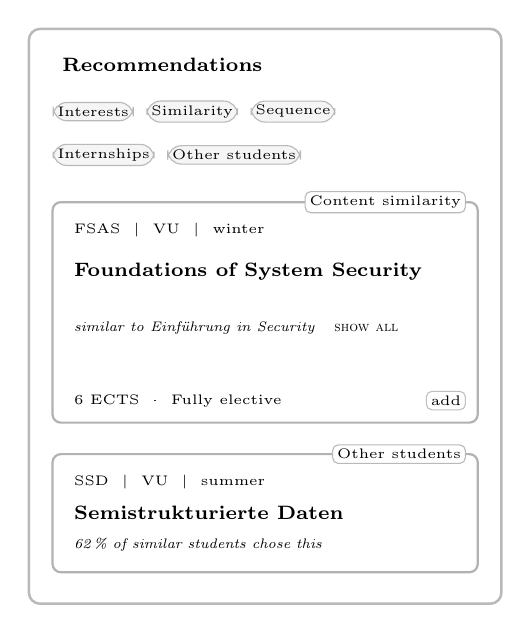
\begin{tikzpicture}[font=\scriptsize,
  chip/.style={draw=gray!55, fill=gray!8, rounded corners=5pt, inner sep=1.6pt, font=\tiny},
  badge/.style={draw=gray!55, fill=white, rounded corners=2pt, inner sep=1.6pt, font=\tiny},
  btn/.style={draw=gray!50, fill=white, rounded corners=2pt, inner sep=1.6pt, font=\tiny}]

  % panel
  \draw[gray!55, line width=0.9pt, rounded corners=4pt, fill=white] (0,0) rectangle (6.0,-7.3);
  \node[font=\scriptsize\bfseries, anchor=west] at (0.3,-0.45) {Recommendations};

  % family toggles
  \node[chip, anchor=west] (t1) at (0.3,-1.05) {Interests};
  \node[chip, anchor=west] (t2) at ([xshift=1.6mm]t1.east) {Similarity};
  \node[chip, anchor=west] (t3) at ([xshift=1.6mm]t2.east) {Sequence};
  \node[chip, anchor=west] (t4) at (0.3,-1.6) {Internships};
  \node[chip, anchor=west] (t5) at ([xshift=1.6mm]t4.east) {Other students};

  % card 1
  \draw[gray!60, line width=0.8pt, rounded corners=3pt, fill=white] (0.3,-5.0) rectangle (5.7,-2.2);
  \node[badge, anchor=east] at (5.55,-2.2) {Content similarity};
  \node[font=\tiny, anchor=west] at (0.45,-2.55) {FSAS \ $|$ \ VU \ $|$ \ winter};
  \node[font=\scriptsize\bfseries, text width=4.9cm, anchor=north west, align=left] at (0.45,-2.85)
    {Foundations of System Security};
  \node[font=\tiny, text width=4.9cm, anchor=north west, align=left] at (0.45,-3.6)
    {\emph{similar to Einführung in Security}\quad \textsc{show all}};
  \node[font=\tiny, anchor=west] at (0.45,-4.72) {6~ECTS \ \textperiodcentered\ \ Fully elective};
  \node[btn, anchor=east] (b1) at (5.55,-4.72) {add};

  % card 2, cropped by the panel edge to show the list scrolls
  \draw[gray!60, line width=0.8pt, rounded corners=3pt, fill=white] (0.3,-6.9) rectangle (5.7,-5.4);
  \node[badge, anchor=east] at (5.55,-5.4) {Other students};
  \node[font=\tiny, anchor=west] at (0.45,-5.75) {SSD \ $|$ \ VU \ $|$ \ summer};
  \node[font=\scriptsize\bfseries, anchor=west] at (0.45,-6.15) {Semistrukturierte Daten};
  \node[font=\tiny, anchor=west] at (0.45,-6.55) {\emph{62\,\% of similar students chose this}};

\end{tikzpicture}
\caption{The Recommendation Panel. Each card names the family that produced it and the reason in the student's own terms, and is draggable into a semester lane; nothing is added to the canvas itself.}
\label{fig:rec-panel}
\end{figure}


This centralised panel represents a deliberate departure from the earlier prototype (Section~\ref{sec:prototype-elicitation}), which relied on per-node actions and floating overlays. A \emph{floating overlay} was rejected because it partially occludes the canvas and forces the user to manage window positions. \emph{Canvas-level annotations} (like pulsing rings on nodes) were rejected for adding visual clutter and risking colour-coding conflicts. A \emph{right-side placement} (tabbed with the Dashboard) was rejected in favour of the left side because recommendations and the catalogue serve the related purpose of finding courses, making adjacent placement more coherent. Regarding the toggles, a \emph{single global on/off switch} was rejected as too coarse for a student who may trust one recommendation family but distrust another, while \emph{hiding inactive families entirely} was rejected because it would prevent students from discovering unused features (e.g., the Internship family).

% ------------------------------------------------------------
\subsection{Accept Flow}
\label{sec:rec-accept}

Accepting a recommendation returns from the Recommendation Panel to the core \emph{Browse $\to$ Shortlist $\to$ Assign} workflow (Section~\ref{sec:workflow}). To satisfy the requirement that accepting a recommendation must not disrupt the user's current context (Feature~\ref{feat:012}, Req.~3), the flow is executed entirely from the spatially independent panel (Section~\ref{sec:rec-panel}). Adding a course from this panel never alters the canvas viewport or node selection state. 
A recommended course is assigned through the same two paths as any other course (Feature~\ref{feat:007}, Req.~6; Section~\ref{sec:interaction-paths}): dragged from its card onto a semester lane, or added through the standard Semester Picker anchored to the card (Section~\ref{sec:semester-picker}). Once a semester is selected by either path, the course immediately transitions to a \emph{parked} or \emph{planned} state. The Compliance Engine re-evaluates the plan, updating the Dashboard. Because a recommendation for a course that is already in the plan is no longer actionable, the accepted card is immediately removed from the panel to keep the active recommendation list clean and focused.

\emph{Retaining accepted cards} (e.g., leaving them visible but greyed out to serve as a history log) was also rejected, as an accumulating list of completed recommendations would quickly clutter the panel.